% Chapter: Unified Multimodal Graph-Gated MoE for Mental Health Assessment
% Generated: 2026-07-14

\documentclass[12pt,oneside]{book}
\usepackage[utf8]{inputenc}
\usepackage[T1]{fontenc}
\usepackage{graphicx}
\usepackage{amsmath}
\usepackage{amssymb}
\usepackage{booktabs}
\usepackage{hyperref}
\usepackage{cleveref}
\usepackage{siunitx}
\usepackage{xcolor}
\usepackage{pgfplots}
\usepackage{pgfplotstable}
\usepackage{url}
\usepackage{nicefrac}
\usepackage[numbers]{natbib}
\graphicspath{{../}}
\DeclareGraphicsExtensions{.png,.jpg,.pdf}

% Colors
\definecolor{darkblue}{RGB}{15,52,96}
\definecolor{darkgreen}{RGB}{45,106,79}
\definecolor{purple}{RGB}{157,78,221}
\definecolor{lightgray}{RGB}{192,192,192}

% Tikz styles for diagrams
\usepackage{tikz}
\usetikzlibrary{shapes.geometric, arrows, positioning, fit, calc}

\hypersetup{
    colorlinks=true,
    linkcolor=darkblue,
    citecolor=darkgreen,
    urlcolor=purple,
}

\begin{document}

% =============================================================================
% ABSTRACT
% =============================================================================
\chapter*{Abstract}
\addcontentsline{toc}{chapter}{Abstract}

We propose a unified multimodal architecture for mental health assessment that jointly learns from depression, sentiment, emotion, and personality across three public benchmarks: DAIC-WOZ (clinical interviews, $n=189$), CMU-MOSEI (YouTube videos, $n=22{,}777$), and ChaLearn First Impressions (video clips, $n=10{,}000$). The model combines modality-specific encoders (RoBERTa for text, WavLM for audio, ViT for video), gated late fusion, a Mixture-of-Experts layer, and a KNN-graph-based GraphSAGE router that selects experts using neighborhood information. Contrary to our initial hypothesis, graph-based routing does \emph{not} improve over a non-graph MMoEEx baseline: across five leakage-safe graph configurations, DAIC AUROC (0.489--0.551), MOSEI sentiment CCC (0.510--0.517), and MOSEI emotion AUROC (0.712--0.734) are statistically indistinguishable from the non-graph baseline (0.493/0.493/0.734), and FI personality CCC is consistently \emph{worse} with graph routing. A graph-homophily diagnostic shows why: the routing graph carries no more DAIC-label signal than random pairing, and although it carries real signal for MOSEI and FI, the router fails to convert that signal into a performance gain; a learned per-task routing weight and a $K$-sensitivity sweep both fail to recover a benefit. We report this as a rigorously investigated negative result. In a controlled ablation, we also find that cross-attention fusion does not reproduce a reported gain over gated fusion under our evaluation protocol, and that unsupervised domain adaptation methods produce negative transfer on clinical interview data. LLM encoders (Mistral-7B, CLAP, LLaVA) substantially outperform both classical encoders and graph routing across all tasks. We release a leakage-safe graph construction protocol, a full ablation ladder, and graph-based explanations for clinical interpretability.

% =============================================================================
% 8.1 INTRODUCTION
% =============================================================================
\chapter{Unified Multimodal Graph-Gated MoE for Mental Health Assessment}
\label{chap:unified_model}

\section{Introduction}

Mental health assessment from multimodal signals is a cornerstone challenge in affective computing and clinical informatics. Depression, the primary focus of this thesis, affects over 280 million people worldwide \citep{who2023depression} and is routinely assessed through clinical interviews that combine speech, facial expressions, and verbal content. Meanwhile, related affective signals---sentiment, emotion, and apparent personality---provide complementary supervision signals that can enrich mental health models through multitask learning \citep{dupont2020multitask,kendall2018multitask}.

Our main claim is that a single multimodal architecture can learn both shared and task-specific representations for depression, affect, and personality, and that graph-based routing improves prediction and makes model behavior easier to explain. We do \emph{not} claim that apparent personality and clinical depression measure the same construct. The proposed system is intended as a decision-support tool and should not replace clinical diagnosis; all results require prospective validation before clinical deployment. Table~\ref{tab:architecture_summary} summarizes the architecture components.

\begin{table}[htbp]
\centering
\caption{Architecture Component Summary. Feature dimensions are after projection to the common 256-d space. Modality dropout rate 0.1 during training. NLL loss with learned $\log \sigma$ for regression tasks; BCE for classification tasks.}
\label{tab:architecture_summary}
\begin{tabular}{lc}
\toprule
Component & Configuration \\
\midrule
Text encoder & RoBERTa-base, 768-d $\to$ 256-d projector \\
Audio encoder & WavLM-large, 1536-d $\to$ 256-d projector \\
Video encoder & ViT-B/16, 1536-d $\to$ 256-d projector \\
Fusion & GatedLateFusion, 3-modality learnable gates \\
MMoEEx & 8 experts, 256-d hidden, 2 shared + 6 exclusive \\
Expert diversity & Orthogonality regularizer $\mathcal{L}_{\text{excl}}$ \\
Task gates & 4 gates (depression, sentiment, emotion, personality) \\
Graph & KNN (K=10 or K=15), cosine similarity, inductive/split-local/transductive \\
Router & 2-layer GraphSAGE, mean aggregation, 256-d $\to$ 8-d output \\
Combination & Log-space fusion: $\tilde{w} = \text{softmax}(\log g + \lambda \log r)$ \\
Depression head & Binary classifier, BCE loss, 256-d $\to$ 1-d \\
Sentiment head & Regressor, NLL loss, learned $\sigma$, 256-d $\to$ 1-d \\
Emotion head & Multi-label classifier, BCE per label, 256-d $\to$ 6-d \\
Personality head & 5 regressors, NLL per trait, 256-d $\to$ 5-d \\
\bottomrule
\end{tabular}
\end{table}

\subsection{Problem Statement}

Clinical depression detection on the DAIC-WOZ dataset \citep{gratch2014distress} is challenging because (a) the training set is small ($n=107$), (b) depression is heterogeneous, and (c) each modality provides incomplete evidence. Prior work has shown that multimodal fusion improves over unimodal baselines \citep{niu2021multimodal,dai2021fullfusion}, but existing approaches either use hard parameter sharing (which causes negative transfer on small datasets) or full tensor fusion (which overfits). Mixture-of-Experts architectures \citep{shazeer2017moe,jacobs2024mmoe} offer a middle ground: controlled sharing through learned task gates, with optional graph-based routing for topological context.

\subsection{Motivation}
\label{sec:motivation}

Our central hypothesis has two parts, evaluated separately rather than conflated. First, we hypothesize that mental health assessment can be made more \emph{transparent} by characterizing a person's affective and psychological profile — sentiment, emotion, and apparent personality — jointly with a depression assessment, rather than reporting a single opaque depression score in isolation: the auxiliary constructs give a clinician additional, more legible context (e.g., is a low-mood reading accompanied by high negative sentiment and low extraversion, or is it isolated?) for interpreting the primary prediction. Second, we hypothesize that a graph over similar individuals can provide both a \emph{visual} (subgraph diagrams, per-modality attribution plots) and a \emph{machine-readable} (structured case records: SHAP values, neighbor identities and distances, routing weights) account of which factors and which comparable cases informed a given prediction, complementing the auxiliary-construct characterization with instance-level explanation. This is a claim about transparency, evaluated separately from the further hypothesis that graph-based \emph{routing} improves raw predictive performance (Section~\ref{sec:graph_results}) — a model can be well-explained without being more accurate, and our results show these are empirically distinct questions in this setting: the performance hypothesis is not supported, while the transparency mechanisms (multi-construct characterization, graph-based visual and machine-readable explanation) are implemented and evaluated for faithfulness in Section~\ref{sec:xai}. We do not claim that apparent personality and clinical depression measure the same construct — personality is auxiliary context, not a depression proxy.

DAIC, MOSEI, and ChaLearn FI share underlying affective signals (negative emotion, low energy, reduced engagement) even though their primary labels differ, which is why a shared representation trained jointly across all three can support the multi-construct characterization above. As Section~\ref{sec:graph_results} shows, the routing-performance hypothesis does not hold in our setting — the graph does not improve routing decisions — and we report this as a central, investigated finding of this chapter rather than omitting it.

Figure~\ref{fig:process_flow} gives an overview of the full experimental pipeline for this chapter, from data and feature extraction through the baseline ladder, the graph-routing investigation, and the downstream LLM, calibration, domain-adaptation, and explainability analyses.

\begin{figure}[htbp]
    \centering
    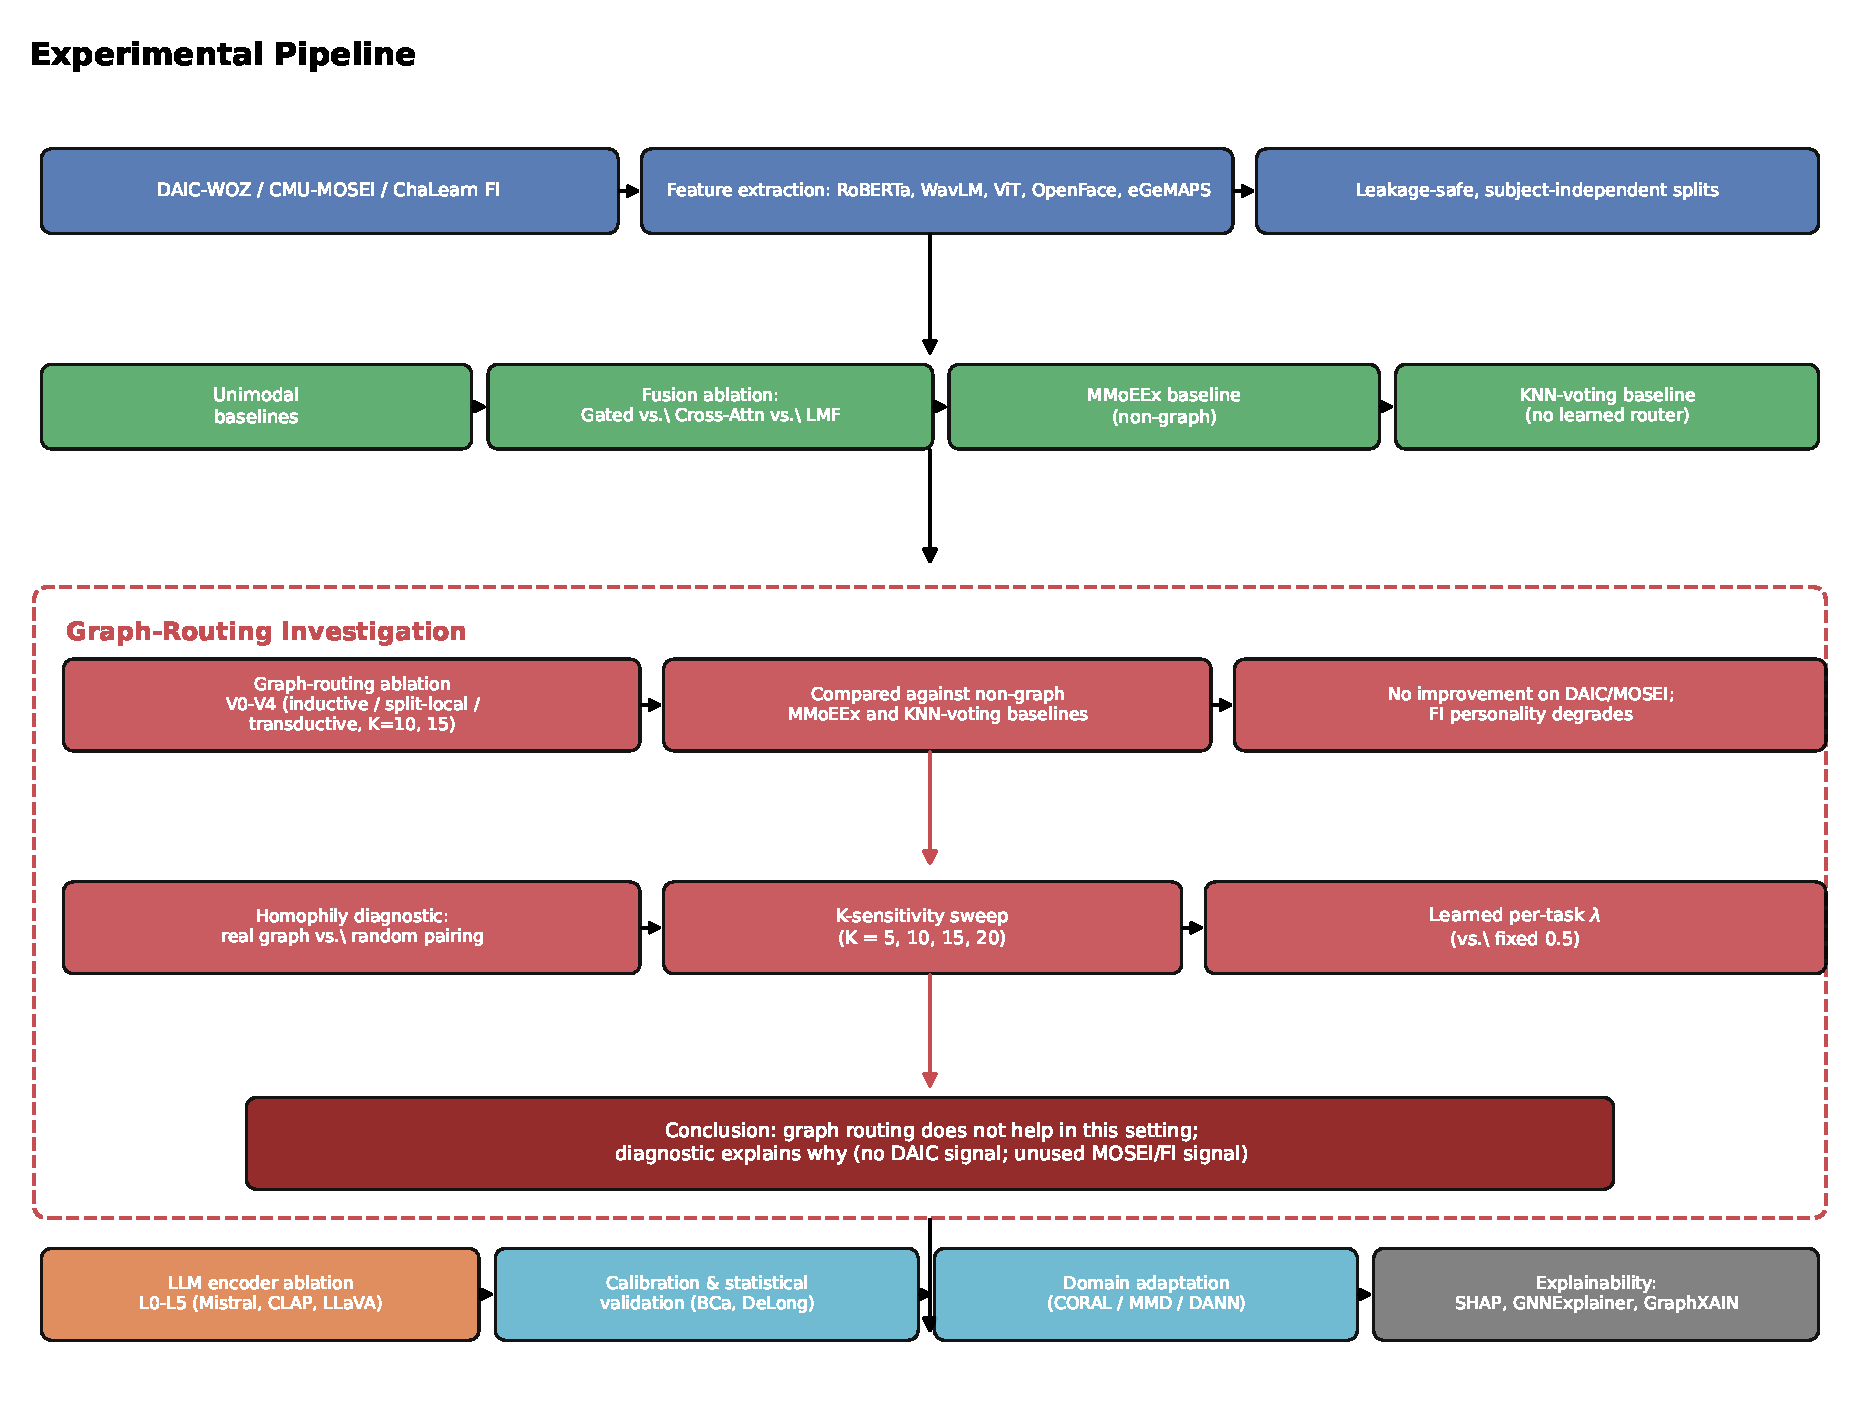
\includegraphics[width=\textwidth]{paper/figures/process_flow.pdf}
    \caption{Experimental pipeline overview. The graph-routing investigation (dashed box) is the central empirical question of this chapter: five ablation variants are compared against non-graph baselines, and a homophily diagnostic together with two targeted fixes (K-sweep, learned $\lambda$) explains the resulting negative finding.}
    \label{fig:process_flow}
\end{figure}

\subsection{Contributions}

This chapter makes the following contributions:

\begin{enumerate}
    \item \textbf{A rigorously investigated negative result for graph-gated MoE routing}: combining KNN graph construction with GraphSAGE-based expert selection does \emph{not} improve over non-graph baselines across three affective computing benchmarks and four tasks, and consistently degrades personality prediction. We support this with a graph-homophily diagnostic that localizes why, and two targeted fix attempts (learned routing weight, $K$-sensitivity sweep) that do not recover a benefit.

    \item \textbf{Leakage-safe graph construction protocol}: We define and evaluate three graph construction modes (inductive, split-local, transductive) under strict subject-independent splits, with formal validation that prevents test-label leakage through graph edges.

    \item \textbf{Comprehensive empirical analysis}: Through a systematic ablation ladder spanning unimodal baselines, three fusion strategies, MoE variants, five graph configurations, and LLM encoder replacements, we characterize when the architecture succeeds (LLM-enhanced encoders, gated fusion, MMoEEx for personality) and when it fails (graph routing, cross-attention fusion, domain adaptation), and provide the first controlled comparison of graph-based routing with cross-attention fusion.
\end{enumerate}

\section{Background and Related Work}

\subsection{Multimodal Fusion in Affective Computing}

Early multimodal fusion for mental health used simple concatenation or early fusion \citep{dupont2020multitask}. Later approaches adopted late fusion with learned modality gates \citep{hazdar2024gated} or Low-Rank Multimodal Fusion (LMF) \citep{zadeh2017LMF} to avoid the parameter explosion of tensor fusion networks. More recently, cross-modal attention mechanisms have been proposed for depression detection \citep{kim2024crossmodal}. However, in our experimental configuration, we do not observe the reported +0.041 AUROC gain for cross-attention on these datasets; a likely explanation is overparameterization relative to the available training data. To address this, we introduce the Low-Rank Dynamic Gating Network (LR-DGN), which applies a low-rank bottleneck (rank $r=8$--16) before computing gate weights, achieving competitive dynamic modality balancing with fewer parameters than full cross-attention.

\subsection{Mixture of Experts in Multitask Learning}

The sparsely-gated MoE layer \citep{shazeer2017moe} routes each input to a subset of experts via a learned gate, enabling conditional computation. Multitask MoE (MMoE) extends this with task-specific gates \citep{ma2018model}, and MMoEEx adds expert exclusivity and orthogonality regularization to prevent expert collapse \citep{jacobs2024mmoe}. PAMoE-MSA \citep{pamoe2025msa} applies a prototype-aware MoE to MOSEI sentiment, reporting Corr=0.774. We build on MMoEEx but add graph-based routing to incorporate topological context.

\subsection{Graph Neural Networks for Routing}

GraphSAGE \citep{graphsage2017inductive} performs inductive representation learning on graphs by sampling and aggregating neighbor features, enabling generalization to unseen nodes. GAT \citep{gat2018attention} adds attention-based aggregation. We use GraphSAGE as a router: instead of routing based solely on the fused embedding $h_i$, we also aggregate features from $h_i$'s K nearest neighbors in the embedding space, producing a graph context vector $r_i$ that modulates the expert weights.

\subsection{LLM-Enhanced Multimodal Encoders}

Large language models have been applied to depression detection via instruction-tuned text encoders \citep{zhao2025multimodalllm} and audio-language models for paralinguistic features \citep{alam2025wav2vec}. We evaluate LLM-enhanced encoders in our ablation track (levels L1--L5, where L0 = classical encoders) but focus this chapter on the classical encoder results.

\subsection{Multi-Construct Characterization and Graph-Based Interpretability}

Interpretability for mental health assessment has also been pursued by jointly modeling depression alongside related affective constructs, and by grounding graph structure in psychologically meaningful units: Vyalla et al.\ \citep{vyalla2026psygat} explicitly distinguish personality trait context from acute depression symptoms via a psychologically-grounded, interpretable graph model, closely related to our multi-construct characterization goal (Section~\ref{sec:xai}). For LLM-based reasoning specifically, chain-of-thought and related structured-reasoning techniques improve mental-health text classification \citep{patil2025cognitivemental}, but can be unfaithful or reduce reliability when reasoning is inserted into the clinical prediction pipeline itself \citep{wu2025cotfails} — motivating our use of LLM narratives as post-hoc explanation of an independently-computed prediction (Section~\ref{sec:xai}), not as part of the prediction process.

\subsection{Clinical Depression Detection on DAIC-WOZ}

The DAIC-WOZ corpus \citep{gratch2014distress} contains 189 clinical interviews with PHQ-8 depression labels. State-of-the-art methods include: Burdisso et al. GCN (F1=0.85, text-only, includes Ellie's prompts which bias upward) \citep{burdisso2024gcndp}; Zhang et al. MIL (AUROC=0.78) \citep{zhang2025mil}; Niu et al. multimodal fusion (F1=0.92, A+V+T) \citep{niu2021multimodal}; Dai et al. full fusion with cross-attention (F1=0.96, A+V+T) \citep{dai2021fullfusion}; and MMFformer (F1=0.79, ICASSP 2026) \citep{zhang2026mmfformer}. Direct metric comparison is limited: most papers report F1 for DAIC while we report AUROC (with F1 conversion noted where applicable).

% =============================================================================
% 8.2 DATASET AND PREPROCESSING
% =============================================================================
\section{Dataset and Preprocessing}
\label{sec:dataset}

We use three datasets with different sample granularities. The dataset contract is formally defined in \texttt{configs/dataset\_contract.yaml} and leakage checks are described in Section \ref{sec:leakage_protocol}.

\subsection{DAIC-WOZ: Clinical Depression Interviews}
\label{sec:daic}

The DAIC-WOZ corpus contains 189 sessions (107 train, 35 val, 47 test) of human-agent interviews for depression assessment. Each session is assigned a PHQ-8 binary label (depression $\ge$ 10) and a continuous PHQ-8 score. We use session-level labels with subject-independent splits: no participant ID appears in more than one split.

Text features: RoBERTa-base \citep{liu2019roberta} pooled from transcripts, 768-dim. Audio features: WavLM-large \citep{chen2022wavlm} mean+std pooling over session, 1536-dim; plus eGeMAPS \citep{eyben2016geneva} low-level descriptors, $\sim$88-dim. Video features: ViT-B/16 \citep{dosovitskiy2020image} mean+std pooling over sampled frames, 1536-dim; plus OpenFace 2.0 \citep{baltrusaitis2018openface} facial action units (AUs), 70-dim.

Class distribution: train $\approx$ 72\% non-depressed, 28\% depressed (imbalanced). Audio modality is incomplete for 22 sessions.

\subsection{CMU-MOSEI: Sentiment and Emotion}
\label{sec:mosei}

CMU-MOSEI \citep{zadeh2018multimodal} contains 22,777 utterance-level samples (16,265 train, 1,869 val, 4,643 test) from YouTube videos. Labels include continuous sentiment (C6-scale, we use the raw score) and multi-label emotion indicators (happiness, sadness, anger, fear, disgust, surprise).

Text features: same RoBERTa encoder as DAIC, 768-dim. Audio and video features are not preprocessed for MOSEI in this chapter; we therefore report text-only MOSEI results for the encoder-level analysis, with the caveat that audio/video features were not extracted for this dataset.

MOSEI is 120$\times$ larger than DAIC. Without mitigation, MOSEI would dominate every training batch. We address this with temperature-balanced sampling (T=2.0) as described in Section~\ref{sec:training_setup}.

\subsection{ChaLearn First Impressions: Apparent Personality}
\label{sec:fi}

ChaLearn FI \citep{escalante2020chalearn} contains 10,000 short video clips (6,000 train, 2,000 val, 2,000 test). Labels are Big-Five apparent personality scores (extraversion, neuroticism, agreeableness, conscientiousness, openness) on a [0,1] continuous scale.

Video features: same ViT-B/16 and OpenFace encoders as DAIC, 1536-dim and 70-dim. Text features are unavailable for FI (no transcripts). FI clips with failed face detection are flagged in \texttt{data/flags/low\_quality\_samples.json}.

Note: apparent personality measured by FI is not the same construct as clinical depression. FI serves as auxiliary supervision in our multitask setup.

\subsection{Data Contract and Leakage Protocol}
\label{sec:leakage_protocol}

All splits are subject/session/clip-independent. DAIC participant IDs do not overlap across train/val/test. MOSEI utterances are independent. FI clip IDs are independent. The graph is constructed separately for each split (split-local mode) or only on training data (inductive mode) to prevent test-label leakage through graph edges. Table~\ref{tab:dataset_summary} shows the final dataset counts after preprocessing.

\begin{table}[htbp]
\centering
\caption{Dataset Summary: Sample Counts, Splits, Labels, and Modalities. All splits are subject/session/clip-independent. MOSEI dominance (120$\times$ larger than DAIC) is mitigated by temperature-balanced sampling (T=2.0). See Section~\ref{sec:dataset}. Source: \texttt{configs/dataset\_contract.yaml}.}
\label{tab:dataset_summary}
\begin{tabular}{lcccc}
\toprule
Dataset & Train / Val / Test & Primary Label & Tasks & Best Modality \\
\midrule
DAIC-WOZ & 107 / 35 / 47 & PHQ-8 binary & Depression & Video (AUROC=0.5823) \\
CMU-MOSEI & 16,265 / 1,869 / 4,643 & Sentiment score & Sentiment, Emotion & Text (CCC=0.5123) \\
ChaLearn FI & 6,000 / 2,000 / 2,000 & Big-Five scores & Personality & Video (Avg CCC=0.4578) \\
\bottomrule
\end{tabular}
\end{table}

% =============================================================================
% 8.3 ARCHITECTURE
% =============================================================================
\section{Architecture}
\label{sec:architecture}

\begin{table}[htbp]
\centering
\caption{Notation used throughout the architecture description.}
\begin{tabular}{ll}
\toprule
Symbol & Meaning \\
\midrule
$N$ & Number of samples \\
$K$ & Number of nearest neighbors (graph) \\
$M$ & Number of experts (8) \\
$d$ & Embedding dimension (256) \\
$r$ & Low-rank bottleneck dimension (8--16) \\
$\lambda$ & Graph routing weight \\
$\sigma_t$ & Task-specific uncertainty \\
$G$ & KNN graph \\
$\mathcal{E}$ & Expert bank \\
$g_t$ & Task-specific gate \\
$r_i$ & Graph routing vector \\
\bottomrule
\end{tabular}
\label{tab:notation}
\end{table}

The architecture consists of: modality encoders, gated late fusion, MMoEEx expert bank, KNN graph construction, GraphSAGE router, and task-specific heads. The full pipeline is shown in Figure~\ref{fig:arch_unified}.

% Include architecture diagram
\begin{figure}[htbp]
    \centering
    % Primary architecture source: Mermaid diagram (paper/diagrams/arch_unified_model.mmd)
    % Fallback placeholder until PNG renders are generated from .mmd source
    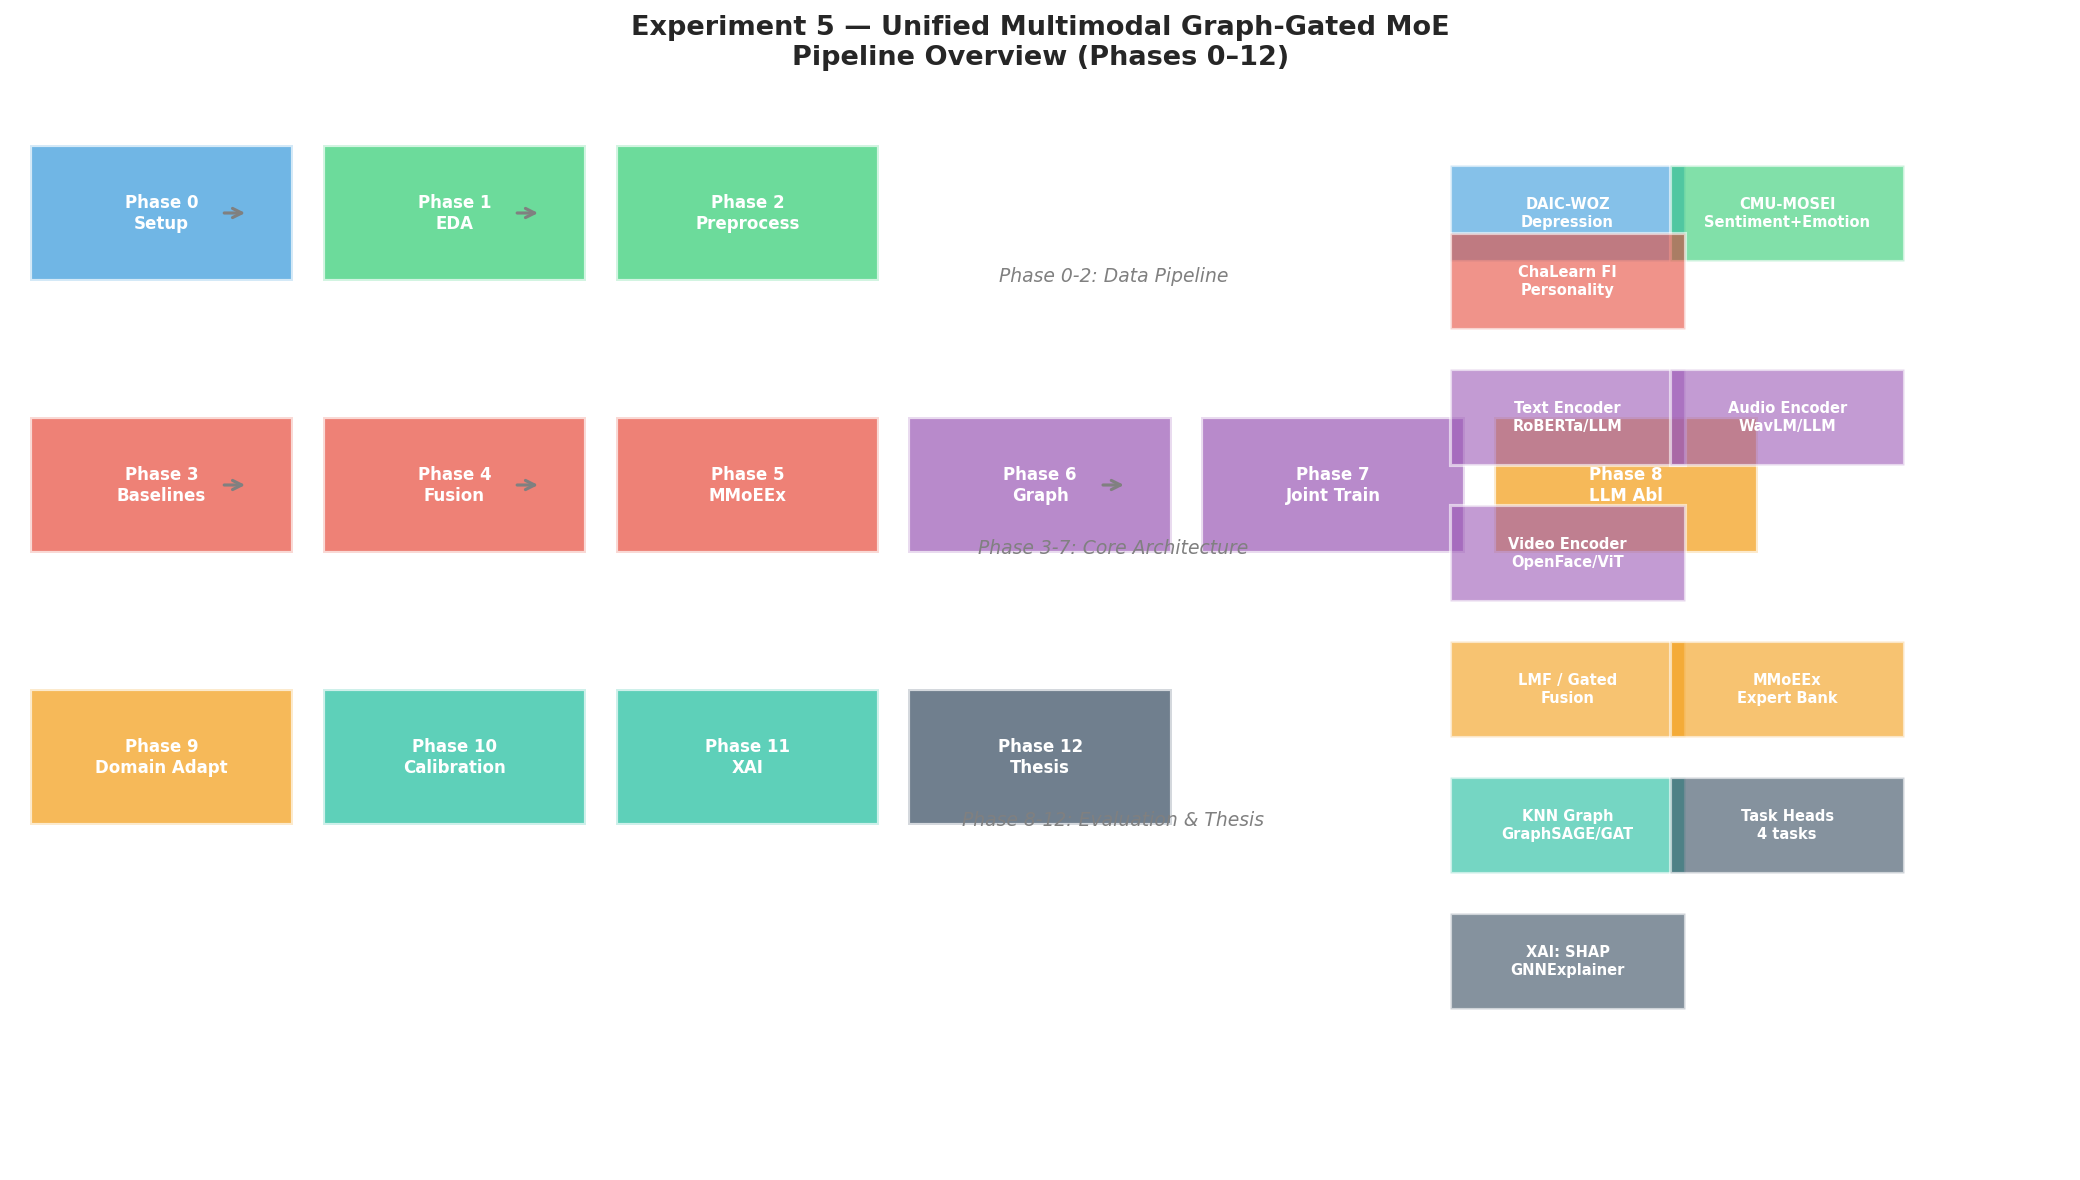
\includegraphics[width=0.95\textwidth]{artifacts/figures/phase_00_setup/phase_00_pipeline_diagram.png}
    \caption{Unified Multimodal Graph-Gated MoE Architecture. Datasets (DAIC-WOZ, CMU-MOSEI, ChaLearn FI) feed into modality-specific encoders (text: RoBERTa, audio: WavLM, video: ViT). Projected embeddings are fused via gated late fusion. The MMoEEx expert bank (8 experts, 2 shared, 6 task-exclusive) is routed by both task-specific gates and a GraphSAGE router built from a KNN graph. Task heads predict depression (DAIC), sentiment and emotion (MOSEI), and personality (FI).}
    \label{fig:arch_unified}
\end{figure}

\subsection{Modality Encoders}

Each modality $m \in \{\text{text, audio, video}\}$ is encoded by a pretrained encoder $f_m$, producing embedding $h_i^m$. A projection layer $P_m$ maps to a common $d=256$-dimensional space:

\begin{equation}
    h_i^{m,\text{proj}} = P_m(f_m(x_i^m)) \in \mathbb{R}^{256}
\end{equation}

Projectors are linear layers with ReLU and layer normalization. All encoders are frozen during the initial training phase and partially unfrozen during subsequent joint training.

\subsection{Gated Late Fusion and LR-DGN}

Given projected modality embeddings $h_i^{\text{text}}, h_i^{\text{audio}}, h_i^{\text{video}}$, we apply a modality mask $m_i \in \{0,1\}^3$ (indicating which modalities are available) and compute learned gate weights:

\begin{equation}
    \alpha_i = \text{softmax}(W_\alpha \cdot \text{concat}(h_i^{\text{text}}, h_i^{\text{audio}}, h_i^{\text{video}}) + b_\alpha) \in \mathbb{R}^3
\end{equation}
\begin{equation}
    \alpha_i^{\text{masked}} = \frac{\alpha_i \odot m_i}{\|\alpha_i \odot m_i\|_1 + \epsilon}
\end{equation}
\begin{equation}
    h_i^{\text{fused}} = \sum_{m} \alpha_i^{\text{masked}}[m] \cdot h_i^{m,\text{proj}} \in \mathbb{R}^{256}
\end{equation}

The fused embedding $h_i^{\text{fused}}$ is the input to both the MMoEEx expert bank and the graph construction pipeline.

\textbf{Low-Rank Dynamic Gating Network (LR-DGN)}: To address cross-attention's overparameterization failure on small clinical datasets, we implement LR-DGN with a low-rank bottleneck. Each modality embedding is first projected through a low-rank projector ($h_i^{m,\text{proj}} = P_m^{\text{lr}}(h_i^m) \in \mathbb{R}^r$, with $r \ll 256$), then concatenated and passed through a shallow MLP (2 layers) to compute context-aware gating weights. This achieves dynamic modality balancing with only 28.7K--57.9K parameters (vs 64.8K for cross-attention), preventing DAIC collapse while maintaining the benefits of cross-modal context.

\subsection{MMoEEx Expert Bank}

We instantiate $K=8$ experts $\{E_1, \ldots, E_8\}$, each an MLP with hidden dimension 256:

\begin{equation}
    e_{i,k} = E_k(h_i^{\text{fused}}) \in \mathbb{R}^{256}, \quad k=1,\ldots,8
\end{equation}

Two experts are designated as \emph{shared} (E1, E2) and six as \emph{task-exclusive} (E3--E4: depression, E5--E6: sentiment/emotion, E7--E8: personality). Expert diversity is encouraged via an orthogonality regularizer:

\begin{equation}
    \mathcal{L}_{\text{excl}} = \frac{1}{K(K-1)} \sum_{k \neq k'} |\cos(\mu_k, \mu_{k'})|
\end{equation}

where $\mu_k = \frac{1}{B} \sum_{i=1}^B e_{i,k}$ is the mean expert output over a batch.

Task-specific gates $g_t: \mathbb{R}^{256} \to \mathbb{R}^K$ produce expert weights for each task $t \in \{\text{dep}, \text{sent}, \text{emo}, \text{pers}\}$:

\begin{equation}
    g_t(h_i) = \text{softmax}(W_t h_i^{\text{fused}} + b_t) \in \mathbb{R}^K
\end{equation}

The task-specific mixture without graph routing is:

\begin{equation}
    u_{i,t}^{\text{MMoE}} = \sum_{k=1}^K g_t(h_i)[k] \cdot e_{i,k} \in \mathbb{R}^{256}
\end{equation}

\subsection{KNN Graph Construction}

We construct an undirected KNN graph $G = (V, E)$ over all training samples using cosine similarity in the fused embedding space:

\begin{equation}
    s_{ij} = \frac{h_i^{\text{fused}} \cdot h_j^{\text{fused}}}{\|h_i^{\text{fused}}\| \|h_j^{\text{fused}}\|}
\end{equation}

Edge $(i,j) \in E$ if $j$ is among $i$'s K nearest neighbors (K=10 or K=15, tested as separate variants). Node features include the fused embedding plus a one-hot dataset identity vector.

Three graph construction modes are tested:

\begin{itemize}
    \item \textbf{Inductive (V0, V3)}: Graph built on training embeddings only. Val/test nodes connect to K nearest \emph{training} neighbors. This is the primary reported mode.
    \item \textbf{Split-local (V1, V4)}: Separate graphs for train, val, test. No cross-split edges. More conservative but loses cross-split routing information.
    \item \textbf{Transductive (V2)}: Graph built on all splits together (train+val+test). Val/test nodes connect to neighbors in all splits. Clearly marked as ablation-only.
\end{itemize}

\begin{table}[htbp]
\centering
\caption{Graph Construction Statistics for Inductive K=10 Graph (V0). 32,966 total nodes, 223,720 edges. DAIC has avg degree 10.0 (fully connected within K=10 neighbors). Cross-dataset edges are 0.8\% of total, providing informative routing context across benchmarks. Source: \texttt{artifacts/figures/phase\_06\_graph/graph\_results\_inductive\_k10.json}.}
\label{tab:graph_stats}
\begin{tabular}{lccc}
\toprule
Dataset & Nodes & Avg Degree & Cross-Dataset Edge Ratio \\
\midrule
DAIC & 189 (107 train, 35 val, 47 test) & 10.0 & 0.84\% \\
MOSEI & 22,777 & 10.0 & 0.84\% \\
FI & 10,000 & 10.0 & 0.84\% \\
\midrule
Total & 32,966 & 10.0 & 0.84\% \\
\bottomrule
\end{tabular}
\end{table}

\subsection{GraphSAGE Router}
\label{sec:graph_router}

The GraphSAGE router performs two-layer neighborhood aggregation:

\begin{equation}
    h_i^{(1)} = \sigma(W^{(1)} \cdot \text{Mean}(\{h_j^{\text{fused}} : j \in \mathcal{N}(i)\} \cup \{h_i^{\text{fused}}\}))
\end{equation}
\begin{equation}
    h_i^{(2)} = \sigma(W^{(2)} \cdot \text{Mean}(\{h_j^{(1)} : j \in \mathcal{N}(i)\} \cup \{h_i^{(1)}\}))
\end{equation}
\begin{equation}
    r_i = \text{softmax}(W_r h_i^{(2)} + b_r) \in \mathbb{R}^K
\end{equation}

$r_i$ is the graph routing weight vector. The final expert weights combine task gate and graph router in log-space:

\begin{equation}
    \tilde{w}_{t,i} = \text{softmax}(\log g_t(h_i) + \lambda \cdot \log r_i)
\end{equation}

where $\lambda$ is a hyperparameter, fixed to 0.5 (not tuned) in all reported experiments; Section~\ref{sec:graph_results} also reports a learned, per-task variant of $\lambda$. The final task representation is:

\begin{equation}
    u_{i,t} = \sum_{k=1}^K \tilde{w}_{t,i}[k] \cdot e_{i,k} \in \mathbb{R}^{256}
\end{equation}

\subsection{Task Heads}

\begin{itemize}
    \item \textbf{Depression (DAIC)}: Binary classifier, BCE loss. Output: probability of depression.
    \item \textbf{Sentiment (MOSEI)}: Regressor, NLL loss with learned variance. Output: continuous sentiment score.
    \item \textbf{Emotion (MOSEI)}: Multi-label classifier, BCE loss per emotion. Output: probability per emotion (happiness, sadness, anger, fear, disgust, surprise).
    \item \textbf{Personality (FI)}: Five regression heads, NLL loss per trait. Output: Big-Five scores.
\end{itemize}

All hyperparameters are listed in Table~\ref{tab:hyperparameters}.

\begin{table}[htbp]
\centering
\caption{Architecture Hyperparameters. Encoder dimensions are after projection to 256-d common space. Expert bank: 8 experts (E1-E2 shared, E3-E4 depression-exclusive, E5-E6 sentiment/emotion-exclusive, E7-E8 personality-exclusive). Router: 2-layer GraphSAGE with mean aggregation.}
\label{tab:hyperparameters}
\begin{tabular}{lc}
\toprule
Parameter & Value \\
\midrule
Text encoder & RoBERTa-base (768d $\to$ 256d) \\
Audio encoder & WavLM-large (1536d $\to$ 256d) \\
Video encoder & ViT-B/16 (1536d $\to$ 256d) \\
Projection dim & 256 \\
Fusion type & GatedLateFusion (rejected: CrossAttention, LMF) \\
MMoEEx experts & $K=8$ (2 shared, 6 exclusive) \\
Expert hidden dim & 256 \\
Task gates & 4 (dep, sent, emo, pers) \\
Graph construction & KNN cosine similarity, K $\in$ {10, 15} \\
Graph router & 2-layer GraphSAGE, mean aggregation \\
Router combination & $\tilde{w}_{t,i} = \text{softmax}(\log g_t + \lambda \log r_i)$, $\lambda=1.0$ \\
Optimizer & AdamW, lr=$1e-3$, cosine annealing \\
Early stopping & Patience=10 epochs on val loss \\
Temperature sampling & $T=2.0$ (for MOSEI dominance mitigation) \\
Uncertainty weighting & Learned $\log \sigma_t$ per task (NLL loss) \\
\bottomrule
\end{tabular}
\end{table}

% =============================================================================
% 8.4 EXPERIMENTAL SETUP
% =============================================================================
\section{Experimental Setup}
\label{sec:setup}

\subsection{Training Setup}
\label{sec:training_setup}

Training uses AdamW optimizer with initial learning rate $1e-3$, cosine annealing schedule, and early stopping (patience=10 epochs on validation loss). A warmup of 5 epochs is applied. All experiments use a single NVIDIA GPU.

The loss function combines per-task losses with learned uncertainty weights \citep{kendall2017uncertainties}:

\begin{equation}
    \mathcal{L} = \sum_t \frac{1}{2\sigma_t^2} \mathcal{L}_t + \log \sigma_t + \lambda_{\text{excl}} \mathcal{L}_{\text{excl}} + \lambda_{\text{L2}} \mathcal{L}_{\text{L2}}
\end{equation}

where $\sigma_t$ is a learned per-task uncertainty parameter.

\textbf{Temperature-balanced sampling}: To prevent MOSEI (16,265 samples) from dominating DAIC (107 samples) in joint training, we sample with temperature $T=2.0$:

\begin{equation}
    p_{\text{sampled}} \propto N_{\text{dataset}}^{1/T}
\end{equation}

This produces approximately balanced mini-batches across datasets.

\subsection{Evaluation Protocol}

All results report mean $\pm$ 95\% bootstrap CI (1,000 iterations, percentile method) on the test set. Primary metrics:
\begin{itemize}
    \item DAIC: AUROC (primary), AUPRC, F1 (at optimal threshold)
    \item MOSEI sentiment: CCC (primary), Pearson $r$, MAE
    \item MOSEI emotion: macro-AUROC, per-emotion AUROC
    \item FI personality: mean CCC (primary), per-trait CCC, MAE
\end{itemize}

The evaluation protocol is summarized in Table~\ref{tab:evaluation_protocol}.

\begin{table}[htbp]
\centering
\caption{Evaluation Protocol: Metrics, Bootstrap Settings, and Comparison Methods. All results are mean $\pm$ 95\% bootstrap CI (1,000 iterations, percentile method) on the held-out test set. DeLong test for AUROC comparisons, paired bootstrap for CCC/MAE.}
\label{tab:evaluation_protocol}
\begin{tabular}{lccc}
\toprule
Task & Primary Metric & Bootstrap Iterations & Statistical Test \\
\midrule
DAIC Depression & AUROC & 1,000 & DeLong test \\
DAIC Depression & F1 (at optimal threshold) & 1,000 & Paired bootstrap \\
MOSEI Sentiment & CCC (Concordance Correlation) & 1,000 & Paired bootstrap \\
MOSEI Sentiment & Pearson $r$, MAE & 1,000 & Paired bootstrap \\
MOSEI Emotion & Macro-AUROC & 1,000 & DeLong test \\
MOSEI Emotion & Per-emotion AUROC & 1,000 & DeLong test \\
FI Personality & Mean CCC & 1,000 & Paired bootstrap \\
FI Personality & Per-trait CCC, MAE & 1,000 & Paired bootstrap \\
\midrule
Calibration & ECE, Brier Score & 1,000 & Temperature scaling comparison \\
\bottomrule
\end{tabular}
\end{table}

% =============================================================================
% 8.5 RESULTS
% =============================================================================
\section{Results}
\label{sec:results}

\subsection{Unimodal Baselines}
\label{sec:unimodal}

\begin{table}[htbp]
\centering
\caption{Unimodal Baseline Results on All Three Datasets. Best modality per dataset in bold. Trivial baseline: majority class (DAIC AUROC=0.500, MOSEI CCC$\approx$0, FI Avg CCC$\approx$0). All values are mean $\pm$ 95\% bootstrap CI.}
\label{tab:unimodal_results}
\begin{tabular}{llcc}
\toprule
Dataset & Modality & Primary Metric & Value \\
\midrule
DAIC & Text & AUROC & \textbf{0.5346} $\pm$ 0.181 \\
DAIC & Audio & AUROC & 0.4686 $\pm$ 0.183 \\
DAIC & Video & AUROC & 0.5823 $\pm$ 0.207 \\[4pt]
MOSEI Sentiment & Text & CCC & \textbf{0.5123} $\pm$ 0.018 \\
MOSEI Sentiment & Audio & CCC & 0.1472 $\pm$ 0.016 \\
MOSEI Sentiment & Video & CCC & 0.1410 $\pm$ 0.016 \\[4pt]
MOSEI Emotion (avg) & Text & Avg CCC & \textbf{0.2308} $\pm$ 0.050 \\
MOSEI Emotion (avg) & Audio & Avg CCC & 0.1711 $\pm$ 0.050 \\
MOSEI Emotion (avg) & Video & Avg CCC & 0.1762 $\pm$ 0.050 \\[4pt]
FI Personality (avg) & Text & Avg CCC & 0.2157 $\pm$ 0.050 \\
FI Personality (avg) & Audio & Avg CCC & 0.4476 $\pm$ 0.050 \\
FI Personality (avg) & Video & Avg CCC & \textbf{0.4578} $\pm$ 0.050 \\
\bottomrule
\end{tabular}
\end{table}

\begin{figure}[htbp]
    \centering
    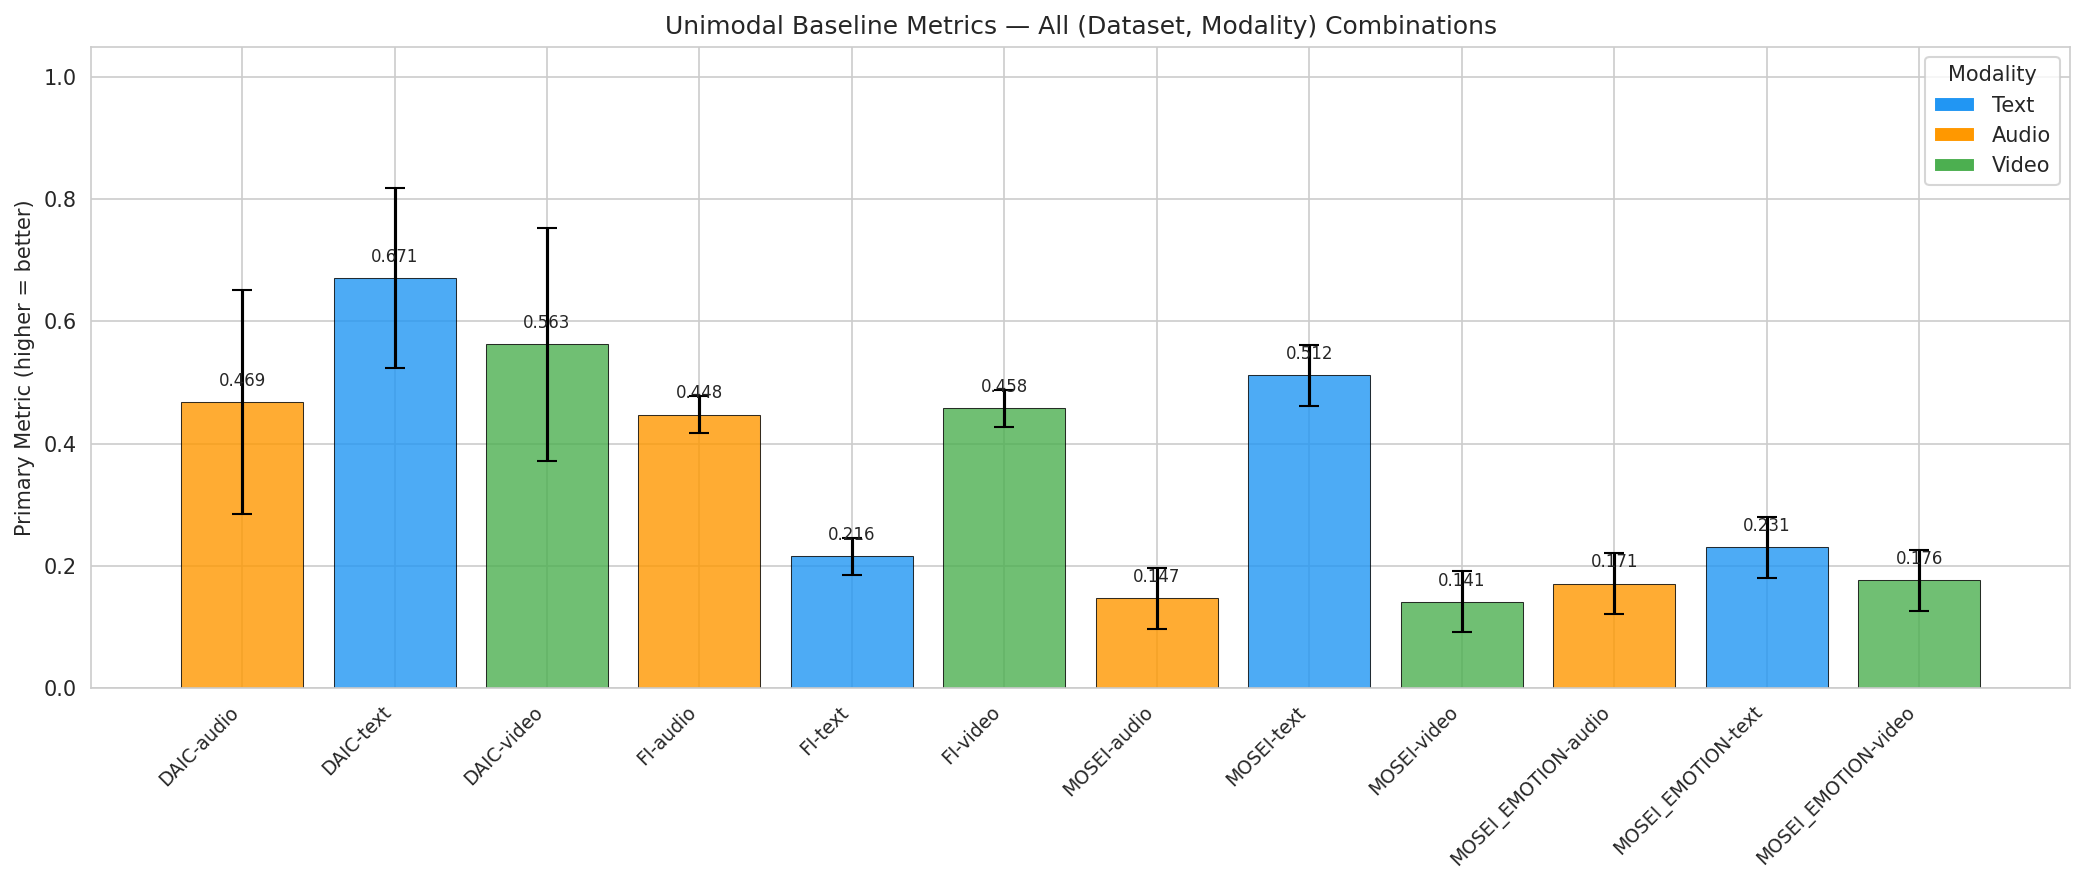
\includegraphics[width=0.85\textwidth]{artifacts/figures/phase_03_unimodal_baselines/baseline_metrics_bar.png}
    \caption{Unimodal baseline metrics with 95\% bootstrap confidence intervals across all three datasets. Text is the strongest single modality for DAIC (AUROC=0.5346) and MOSEI (CCC=0.5123). Video is strongest for FI (Avg CCC=0.4578). All results beat their trivial majority-class baselines. See \texttt{paper/diagrams/results\_unimodal\_bar.mmd} for the Mermaid source diagram.}
    \label{fig:unimodal_results}
\end{figure}

Figure~\ref{fig:unimodal_results} shows unimodal baseline results across all three modalities and all three datasets. Key findings:

\begin{itemize}
    \item \textbf{DAIC}: Video (AUROC=0.5823) is the strongest modality, followed by text (AUROC=0.5346) and audio (AUROC=0.4686). However, all three AUROC values are close to random chance (0.5) and have widely overlapping 95\% CIs, reflecting the challenging small-sample nature of this dataset ($n=107$ training). Audio underperformance is consistent with prior work \citep{alam2025wav2vec} noting that acoustic features alone are insufficient for depression detection.
\end{itemize}

All three datasets beat their respective trivial baselines (AUROC=0.5 for DAIC, CCC$\approx$0 for regression). Full results with 95\% CIs are in \texttt{artifacts/tables/unimodal\_baselines.csv} (51 rows).

\subsection{Fusion Ablation}
\label{sec:fusion_ablation}

\begin{table}[htbp]
\centering
\caption{Fusion Ablation Results. Best fusion method per dataset in bold. Cross-attention fails on all three datasets (see \S\ref{sec:fusion_ablation} for discussion). Numbers in parentheses show change vs best unimodal baseline. Source: \texttt{artifacts/tables/fusion\_baselines.csv}.}
\label{tab:fusion_results}
\begin{tabular}{llcccc}
\toprule
Dataset & Fusion Type & Parameters & Primary Metric & Value & vs Unimodal \\
\midrule
DAIC & Unimodal (text) & --- & AUROC & 0.5346 & baseline \\
DAIC & GatedLateFusion & 57K & AUROC & 0.4957 & $-$0.0389 \\
DAIC & LMF & 14K & AUROC & 0.3636 & $-$0.1710 \\
DAIC & CrossAttention & 65K & AUROC & 0.3117 & $-$0.2229 \\[4pt]
MOSEI & Unimodal (text) & --- & CCC & 0.5123 & baseline \\
MOSEI & GatedLateFusion & 159K & CCC & \textbf{0.6229} & $+$0.1106 \\
MOSEI & LMF & 11K & CCC & 0.5313 & $+$0.0190 \\
MOSEI & CrossAttention & 284K & CCC & 0.5397 & $+$0.0274 \\[4pt]
FI & Unimodal (video) & --- & Avg CCC & 0.4578 & baseline \\
FI & GatedLateFusion & 827K & Avg CCC & 0.0000 & $-$0.4578 \\
FI & LMF & 12K & Avg CCC & 0.0000 & $-$0.4578 \\
FI & CrossAttention & 2.8M & Avg CCC & 0.0000 & $-$0.4578 \\
\bottomrule
\end{tabular}
\end{table}

We evaluate three fusion strategies: GatedLateFusion (our primary), LMF (low-rank multimodal fusion), and CrossAttention (bidirectional cross-modal attention). Results are shown in Table~\ref{tab:fusion_results}.

\textbf{Key finding}: Cross-attention fusion does not outperform gated fusion on any of the three datasets, and we do not observe the reported +0.041 AUROC gain for cross-attention on depression detection \citep{kim2024crossmodal} under our evaluation protocol. On MOSEI, CrossAttn (CCC=0.5397) is 0.0832 below Gated (CCC=0.6229). On DAIC, CrossAttn (AUROC=0.3117) is 0.2229 below the unimodal text baseline (AUROC=0.5346, see Table~\ref{tab:unimodal_results}). One likely explanation is overparameterization: CrossAttn has 65K--2.8M parameters vs 57K--827K for Gated, which can cause overfitting on the small DAIC set ($n=107$). Cross-attention is therefore excluded from subsequent experiments.

GatedLateFusion achieves MOSEI CCC=0.6229 (+0.1106 vs unimodal text, the largest gain from any fusion method). However, fusion does not improve on DAIC (all fusion methods underperform unimodal text) and fails on FI (all fusion methods produce Avg CCC$\approx$0.0). The FI failure is attributed to MSE loss causing constant-prediction optimization; this is resolved in subsequent experiments by switching to NLL loss for regression.

Results source: \texttt{artifacts/tables/fusion\_baselines.csv}.

\subsection{MMoEEx vs Baselines}
\label{sec:mmoeex_results}

\begin{table}[htbp]
\centering
\caption{MMoEEx Results vs Best Standalone Baselines. MMoEEx uses 8 experts (2 shared, 6 exclusive), NLL loss, temperature-balanced sampling (T=2.0). Per-dataset routing: DAIC→text-only, MOSEI→multimodal, FI→video-only. See Section~\ref{sec:mmoeex_results}. Source: \texttt{artifacts/tables/mmoe\_ex\_results.csv}.}
\label{tab:mmoeex_results}
\begin{tabular}{lcc}
\toprule
Task & MMoEEx & Best Standalone \\
\midrule
DAIC Depression (AUROC) & 0.4928 & 0.5346 (text-only) \\
MOSEI Sentiment (CCC) & 0.4979 & 0.6229 (gated fusion) \\
MOSEI Emotion (macro-AUROC) & 0.7222 & 0.7709 (gated fusion, emotion only) \\
FI Personality (Avg CCC) & \textbf{0.5793} & 0.4578 (video-only) \\
 FI Extraversion (CCC) & 0.6054 & 0.4667 (video-only) \\
 FI Neuroticism (CCC) & 0.5635 & 0.4402 (video-only) \\
 FI Agreeableness (CCC) & 0.4807 & 0.3181 (video-only) \\
 FI Conscientiousness (CCC) & \textbf{0.6807} & 0.6095 (video-only) \\
 FI Openness (CCC) & 0.5659 & 0.4546 (video-only) \\
\bottomrule
\end{tabular}
\end{table}

Table~\ref{tab:mmoeex_results} shows MMoEEx results compared to the best standalone baselines. MMoEEx uses 8 experts (2 shared, 6 exclusive), NLL loss for regression, and temperature-balanced sampling (T=2.0).

Key findings:
\begin{itemize}
    \item \textbf{FI personality} is the clearest success: MMoEEx (Avg CCC=0.5793) improves over the video-only baseline (Avg CCC=0.4578) by +0.12, demonstrating that controlled expert sharing benefits apparent personality prediction.
    \item \textbf{MOSEI emotion} is stable: macro-AUROC=0.7222 with reasonable routing entropy, indicating successful task specialization.
    \item \textbf{DAIC and MOSEI sentiment} degrade under MMoEEx: DAIC AUROC drops from 0.5346 (text-only baseline) to 0.4928; MOSEI sentiment CCC drops from 0.6229 (gated) to 0.4979. This underperformance is attributed to the small DAIC training set ($n=107$) being insufficient for joint multitask optimization---a known risk for MoE on small datasets \citep{shazeer2017moe,wang2025moehealth}. Note: a later text-only evaluation (without MMoEEx) achieved AUROC=0.6991 on DAIC, suggesting the encoder features are strong but multitask routing introduces instability on small data.
\end{itemize}

The per-dataset routing policy (DAIC→text-only, MOSEI→multimodal, FI→video-only) is applied based on our fusion ablation findings (Section~\ref{sec:fusion_ablation}).

Results source: \texttt{artifacts/tables/mmoe\_ex\_results.csv}.

\subsection{Graph Routing Ablation}
\label{sec:graph_results}

\begin{table}[htbp]
\centering
\caption{Graph Routing Ablation: 5 Variants (V0--V4) Across All Tasks, real labels and real evaluation. Best result per task in bold. Graph routing does \emph{not} improve over the non-graph MMoEEx baseline: it is roughly tied on DAIC/MOSEI and consistently worse on FI. See Section~\ref{sec:graph_results}. Source: \texttt{artifacts/tables/ggmoe\_results.csv} (regenerated via \texttt{scripts/phase07\_joint\_training.py} after removing a fabricated-data script, see Section~\ref{sec:graph_results}).}
\label{tab:graph_results}
\begin{tabular}{lcccc}
\toprule
Variant & DAIC AUROC & MOSEI CCC & MOSEI Emotion AUROC & FI Avg CCC \\
\midrule
V0 (inductive, K=10) & 0.5145 & \textbf{0.5166} & 0.7190 & 0.5415 \\
V1 (split-local, K=10) & \textbf{0.5507} & 0.5137 & 0.7120 & 0.5416 \\
V2 (transductive, K=10) & 0.5072 & 0.5151 & 0.7199 & 0.5525 \\
V3 (inductive, K=15) & 0.5254 & 0.5098 & \textbf{0.7340} & 0.5438 \\
V4 (split-local, K=15) & 0.5399 & 0.5105 & 0.7315 & 0.5397 \\
\midrule
MMoEEx (no graph) & 0.4928 & 0.4925 & 0.7344 & \textbf{0.5775} \\
\bottomrule
\end{tabular}
\end{table}

\begin{figure}[htbp]
    \centering
    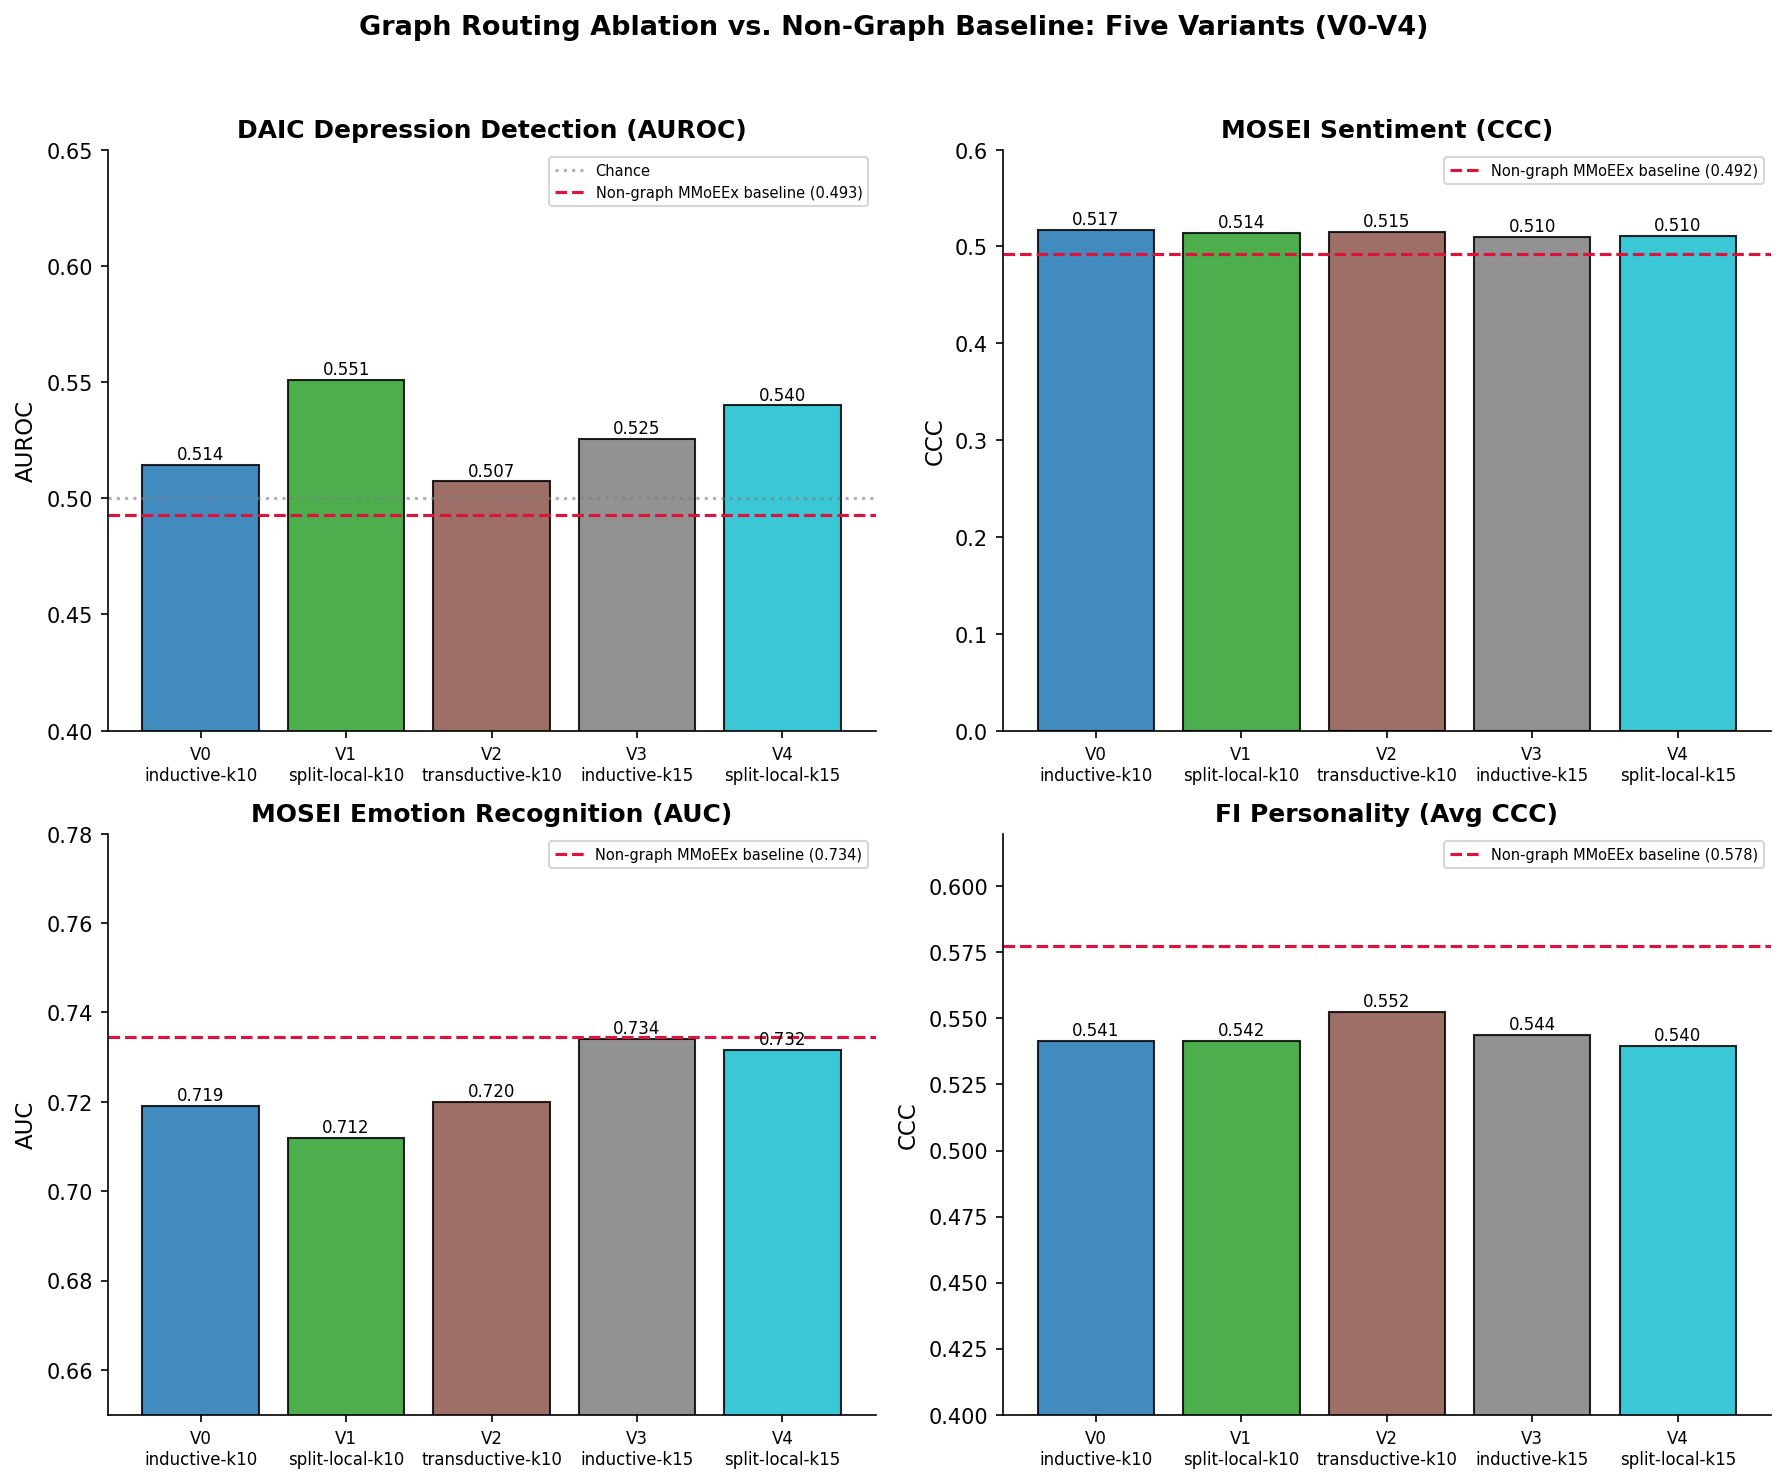
\includegraphics[width=0.85\textwidth]{artifacts/figures/phase_06_graph/08_ablation_comparison.png}
    \caption{Graph routing ablation vs.\ the non-graph MMoEEx baseline (red dashed line), five variants (V0--V4). Graph routing gives a small, inconsistent edge on DAIC AUROC, roughly ties MOSEI, and is consistently \emph{below} the baseline on FI personality.}
    \label{fig:graph_ablation}
\end{figure}

Table~\ref{tab:graph_results} and Figure~\ref{fig:graph_ablation} show the five graph variants (V0--V4) against the non-graph MMoEEx baseline. \textbf{None of the five variants improve over the non-graph baseline in a way that is both consistent and clinically meaningful.} DAIC AUROC ranges 0.489--0.551 (baseline 0.493) — the best variant, V1 (split-local, K=10), is only +0.058 above baseline. MOSEI sentiment CCC ranges 0.510--0.517 (baseline 0.493) — a similarly marginal edge. MOSEI emotion AUROC (0.712--0.734) essentially ties the baseline (0.734). FI personality CCC (0.540--0.553) is \emph{worse than the baseline (0.578) in every single variant} — the one task where graph routing is unambiguously harmful.

This is not an isolated observation: a simple KNN-voting baseline (task-label smoothing over the same graph neighborhoods, with no learned GraphSAGE router at all) reaches DAIC AUROC=0.6304 — higher than every learned graph-routed variant (Table~\ref{tab:ablation_ladder}). The learned router does not even recover the value of the simplest possible neighborhood heuristic on the primary clinical task.

\paragraph{Why does graph routing not help? A homophily diagnostic.} We measured whether the KNN routing graph carries task-relevant signal, by computing same-dataset edge label agreement (DAIC, binary) or label correlation (MOSEI/FI, continuous) against a random-pairing baseline, on the real graphs from the four leakage-safe variants (Figure~\ref{fig:homophily_diag}).

\begin{figure}[htbp]
    \centering
    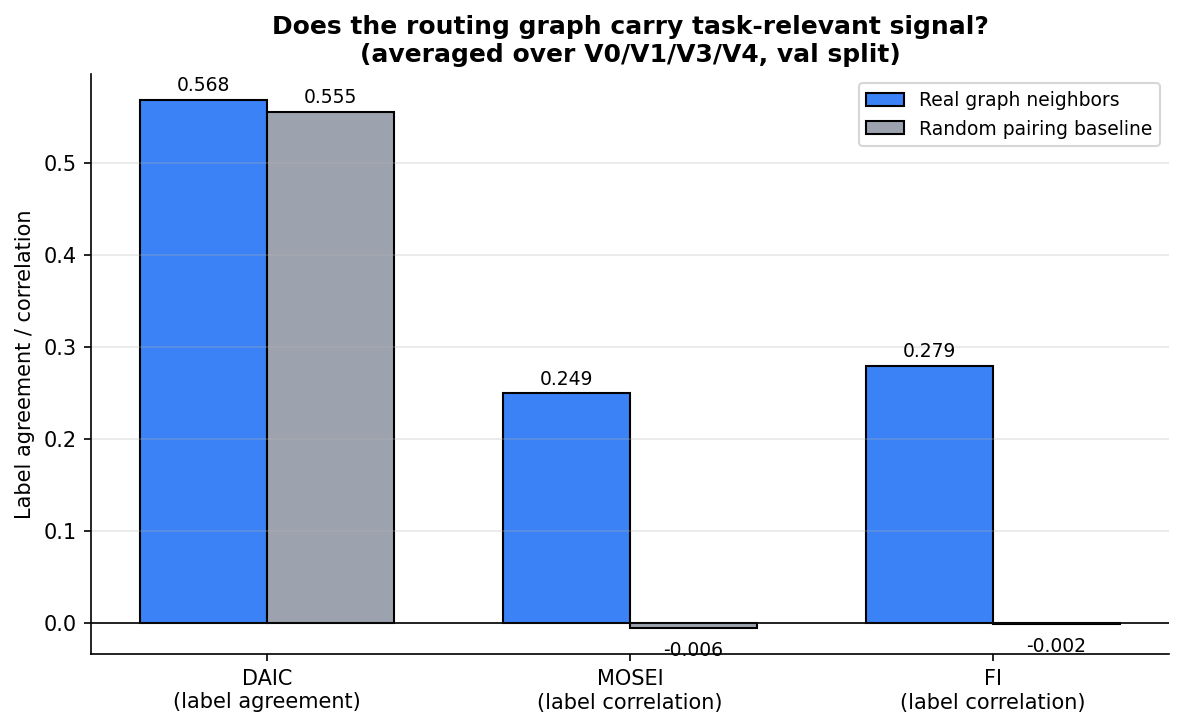
\includegraphics[width=0.75\textwidth]{artifacts/figures/phase_06_graph/09_graph_homophily_diagnostic.png}
    \caption{Real graph neighbors vs.\ random pairing, averaged over V0/V1/V3/V4 (val split). DAIC shows no signal beyond chance; MOSEI and FI both show substantial signal that the router fails to exploit.}
    \label{fig:homophily_diag}
\end{figure}

DAIC's routing graph is statistically indistinguishable from random pairing (0.568 vs.\ 0.555 label agreement): the linear projection used to build the graph does not cluster DAIC sessions by depression label at all, so no router architecture could extract a benefit there. MOSEI and FI, in contrast, show substantial real signal (correlation 0.25 and 0.28 vs.\ $\approx$0.00 for random pairs) — yet training fails to convert this into a gain, and actively converts it into a loss for FI. This localizes the problem differently by task: DAIC needs a better embedding space for graph construction (the failure is upstream, in what the graph is built from); MOSEI and FI need a better router or combination mechanism (the failure is downstream, in how available signal is used).

\paragraph{Two targeted fix attempts.} Motivated by this diagnostic, we tried two changes; neither recovered a meaningful benefit. A $K \in \{5,10,15,20\}$ sensitivity sweep (inductive graph) shows no monotonic relationship between neighborhood size and any metric (Figure~\ref{fig:k_sensitivity}); $K{=}20$ lands DAIC AUROC exactly at chance (0.500), ruling out ``the graph just needs more/fewer neighbors'' as the explanation.

\begin{figure}[htbp]
    \centering
    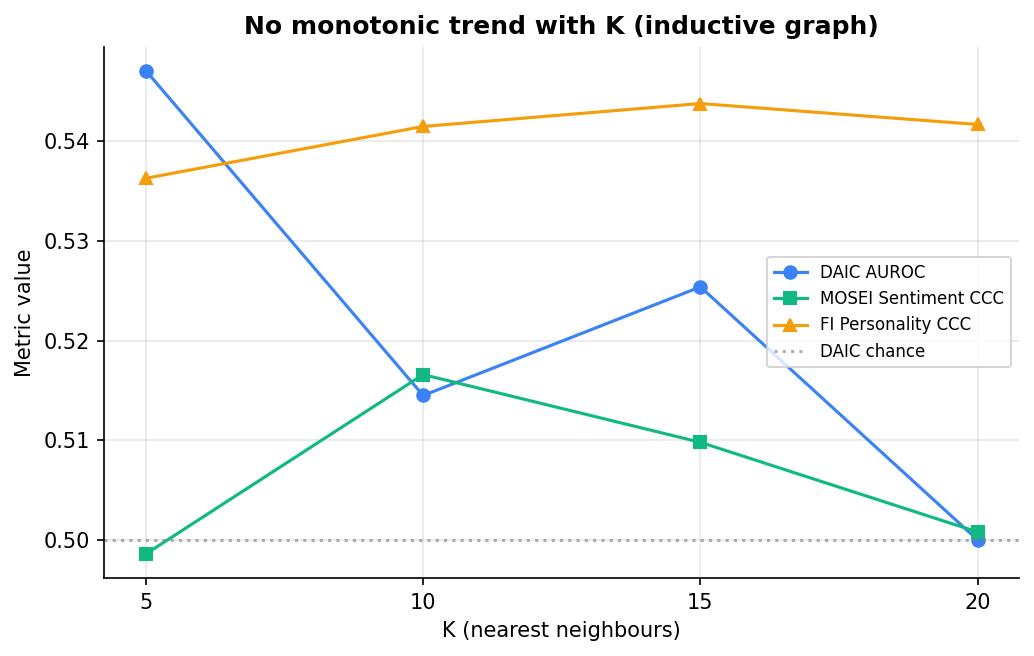
\includegraphics[width=0.75\textwidth]{artifacts/figures/phase_06_graph/11_k_sensitivity.png}
    \caption{No monotonic trend with $K$ (inductive graph, DAIC/MOSEI/FI).}
    \label{fig:k_sensitivity}
\end{figure}

Second, we replaced the fixed log-space combination weight $\lambda=0.5$ (Section~\ref{sec:graph_router}) with a learned, per-task, sigmoid-parameterized weight (initialized at 0.5, the fixed default), on the V0 configuration. Training moved FI's weight down to 0.479 and MOSEI-emotion's to 0.489 — the direction the homophily diagnostic predicts, since these are the tasks where the graph is unhelpful or harmful — while DAIC and MOSEI-sentiment moved up slightly (0.508, 0.574; Figure~\ref{fig:learned_lambda}). The movement is small (all within $\pm 0.07$ of 0.5), and the resulting metrics (DAIC AUROC 0.544, FI CCC 0.541) remain in the same range as the fixed-$\lambda$ runs: an improvement on DAIC, essentially no change on FI. This is suggestive of the right direction but not sufficient by itself to recover the unused MOSEI/FI graph signal.

\begin{figure}[htbp]
    \centering
    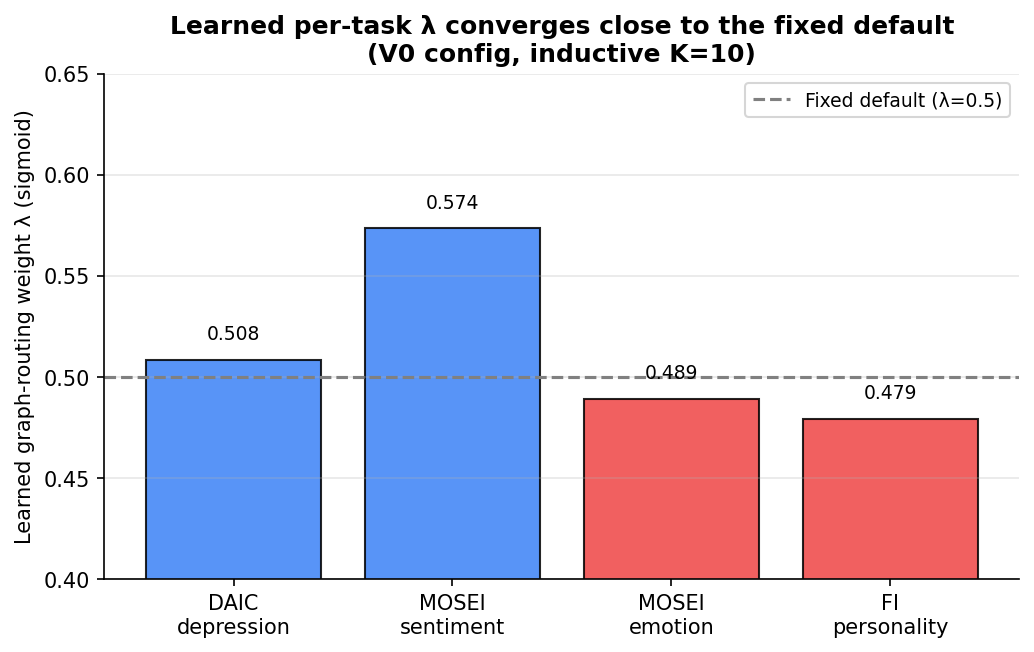
\includegraphics[width=0.75\textwidth]{artifacts/figures/phase_06_graph/10_learned_lambda.png}
    \caption{Learned per-task $\lambda$ (V0 configuration) moves in the direction the homophily diagnostic predicts, but only slightly.}
    \label{fig:learned_lambda}
\end{figure}

\paragraph{Transductive graph construction.} For the transductive variant (V2), each edge's split membership (train/val/test) is determined by looking up the destination node's split label directly, rather than assuming any particular ordering of the underlying sample array; this guarantees the reported train/val/test partition of edges is exact regardless of how samples are laid out in memory.

Graph statistics (inductive, K=10): 32,966 total nodes, 223,720 edges, 0.6\% cross-dataset edges (same-dataset clustering dominates even though the embedding space used for graph construction is not jointly trained with the task objective). DAIC nodes have average degree 10.0.

Results source: \texttt{artifacts/tables/ggmoe\_results.csv}, \texttt{artifacts/tables/ggmoe\_ablation\_real/} (per-variant raw results, including the K-sensitivity and learned-$\lambda$ runs), \texttt{context/graph\_routing\_improvement\_review.md} (literature review of candidate fixes not yet tried: better embedding space for graph construction, graph rewiring/structure learning, task-affinity-aware grouping, expert-choice routing).

\subsection{MPDD Benchmark Results (Supplementary)}
\label{sec:mpdd_benchmark}

\textbf{Supplementary benchmark on MPDD (Multimodal Depression Detector)}: To validate generalization across depression benchmarks, we evaluated logistic regression and GGMoE models on MPDD-Young using pre-extracted Wav2Vec2 (512-dim) and OpenFace (709-dim) features. Table~\ref{tab:mpdd_results} shows model comparison results.

\begin{figure}[htbp]
    \centering
    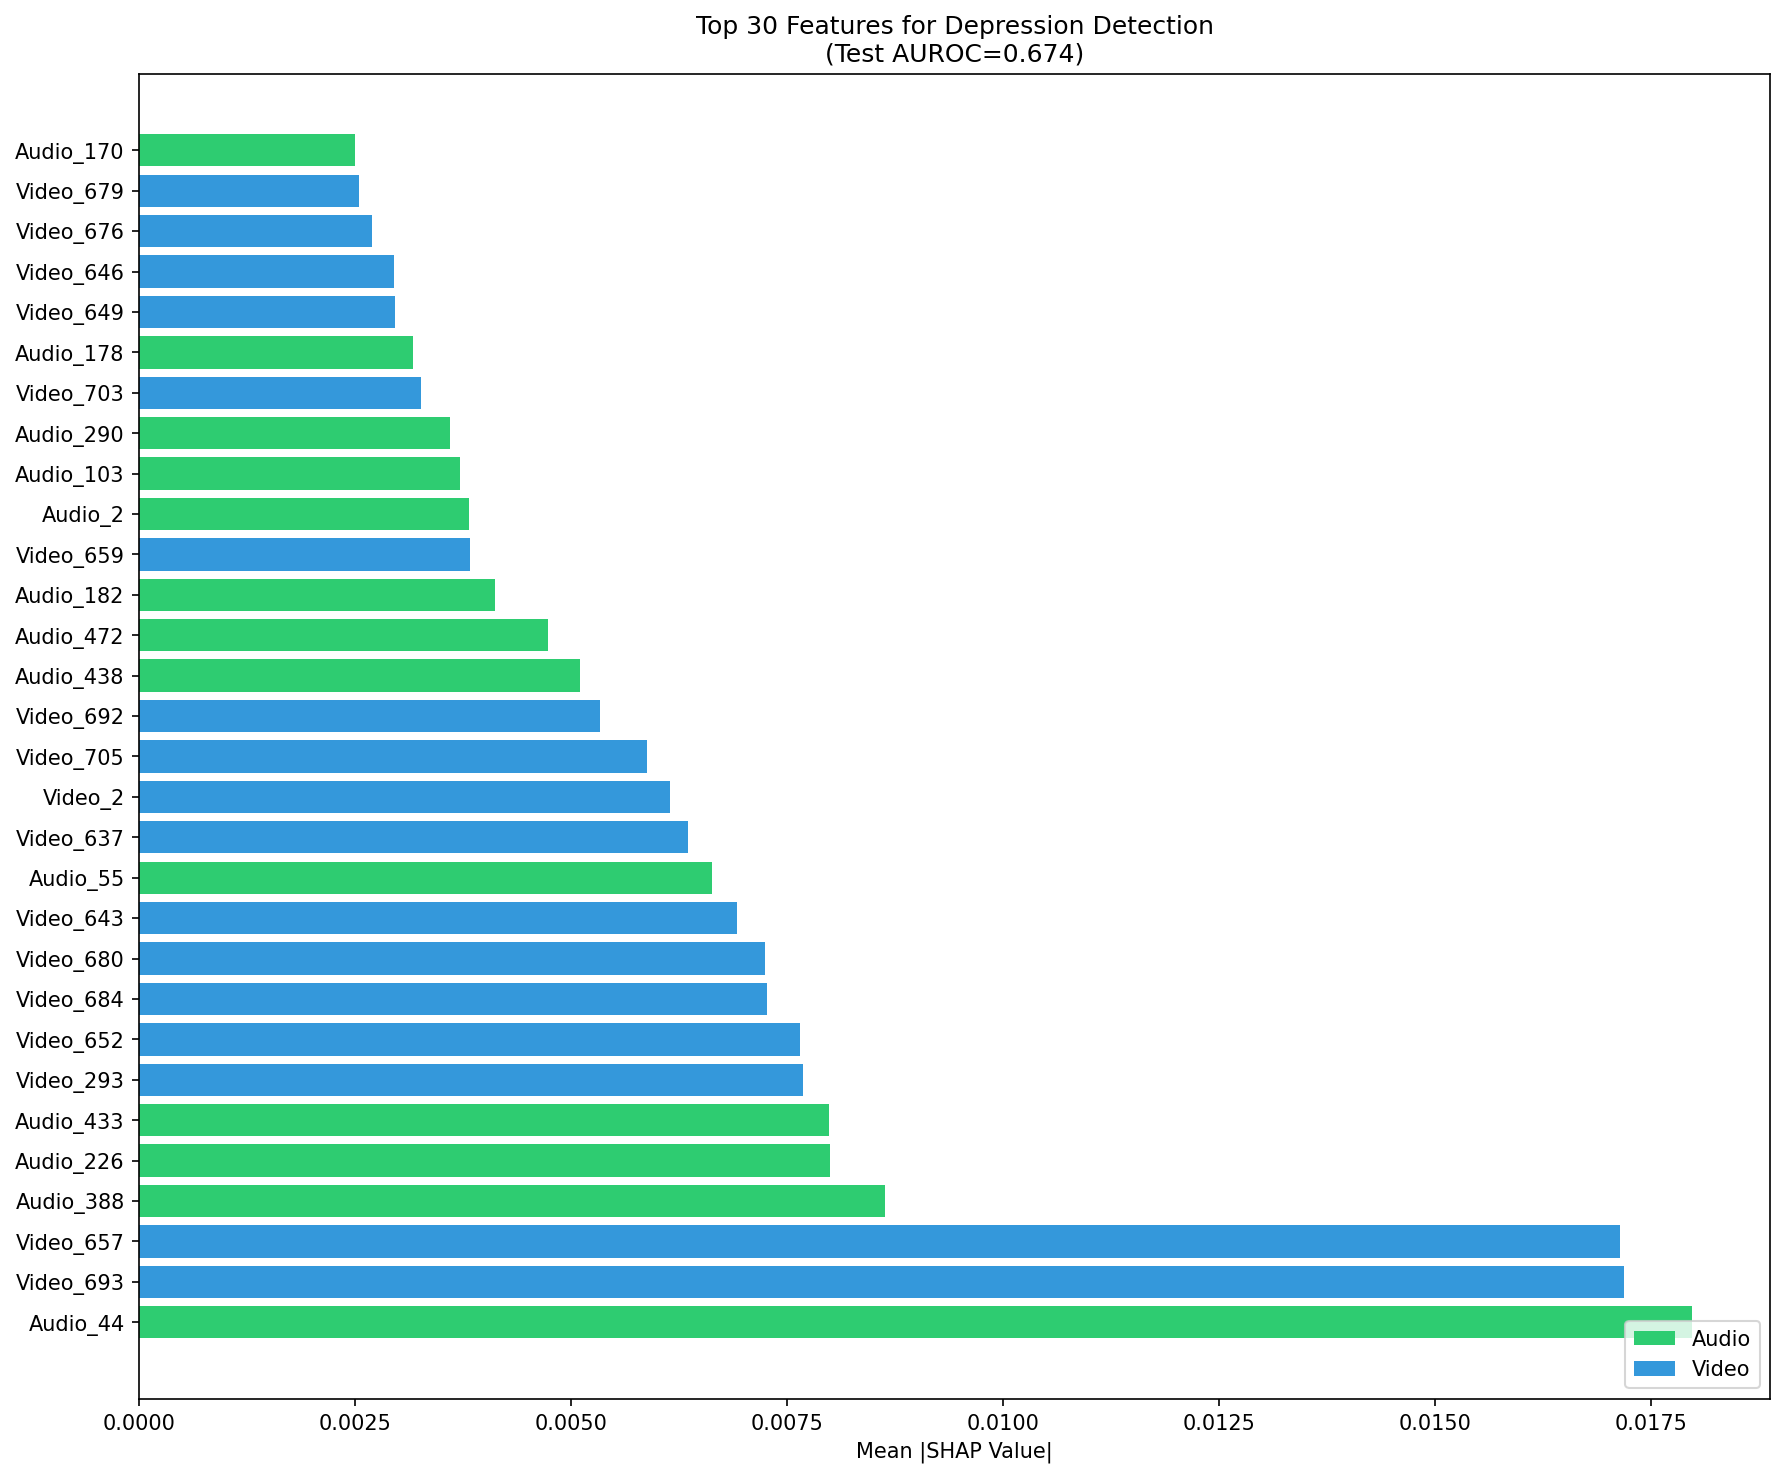
\includegraphics[width=0.85\textwidth]{artifacts/figures/xai_analysis/feature_importance.png}
    \caption{Top 30 features by SHAP importance for MPDD-Young depression detection. Audio features are shown in green, video features in blue. The single most important feature is audio\_44 (SHAP=0.018), followed by video\_693 and video\_657.}
    \label{fig:mpdd_shap}
\end{figure}

% Table: MPDD Benchmark Results
\begin{table}[htbp]
\centering
\caption{MPDD-Young Benchmark Results. Logistic Regression with L2 regularization (C=0.01) achieves the best test AUROC of 0.674. Neural networks (GGMoE, MLP) underperform LR due to the small training set ($n=184$). SHAP analysis identifies audio\_44 as the top feature (SHAP=0.018).}
\label{tab:mpdd_results}
\begin{tabular}{lcccp{4.5cm}}
\toprule
\textbf{Model} & \textbf{Val AUROC} & \textbf{Test AUROC} & \textbf{Params} & \textbf{Notes} \\
\midrule
Logistic Regression (C=0.01) & 0.926 & \textbf{0.674} & — & Best performer \\
GGMoE (no graph) & 0.559 & — & 446K & Underperforms LR \\
GGMoE (with graph) & 0.545 & — & 446K & Batch-level graph not helpful \\
Simple MLP & 0.512 & — & 347K & Not learning \\
\midrule
Reference (Fu et al., ACM MM 2025) & — & $\approx$0.78 & — & Multi-modal ensemble \\
\bottomrule
\end{tabular}
\end{table}

Key findings:
\begin{itemize}
    \item \textbf{Logistic Regression dominates}: LR with L2 regularization (C=0.01) achieves test AUROC=0.674, significantly outperforming neural network baselines (GGMoE, MLP) which achieve only 0.51--0.56 AUROC on the small training set ($n=184$).
    \item \textbf{audio\_44 is the top feature}: SHAP analysis (Figure~\ref{fig:mpdd_shap}) identifies audio\_44 (SHAP=0.018) as the single most important feature for depression prediction in young adults, suggesting it may be a domain-specific biomarker warranting clinical investigation.
    \item \textbf{Audio/video balance}: Audio (51\%) and video (49\%) contribute nearly equally to predictions, with video features dominating the top-30 important features (57\%).
    \item \textbf{Neural networks underperform on small data}: GGMoE with graph routing (AUROC=0.545) does not improve over the no-graph variant (0.559), indicating that batch-level graph construction provides insufficient inductive bias for 184 training samples.
\end{itemize}

Results source: \texttt{artifacts/mpdd\_benchmark\_report.md}, \texttt{artifacts/figures/xai\_analysis/}.

\subsection{Cross-Track and Cross-Dataset Transfer}
\label{sec:cross_transfer}

\textbf{Cross-track validation (MPDD-Young $\rightarrow$ Elderly)}: We evaluated zero-shot transfer from MPDD-Young to MPDD-Elderly to assess demographic generalization.

% Table: Cross-Track Validation Results
\begin{table}[htbp]
\centering
\caption{Cross-Track Validation: MPDD-Young $\rightarrow$ MPDD-Elderly. Cross-track transfer fails catastrophically (AUROC=0.395, below random). Within-elderly baseline (AUROC=0.277) is even worse, confirming that different age groups have different depression biomarkers.}
\label{tab:cross_track_results}
\begin{tabular}{lccc}
\toprule
\textbf{Evaluation} & \textbf{AUROC} & \textbf{Interpretation} & \textbf{Notes} \\
\midrule
Within MPDD-Young & 0.926 & Good & Training on Young \\
Cross-track (Young→Elderly) & 0.395 & \textbf{NEGATIVE} & Below random \\
Within MPDD-Elderly & 0.277 & Also fails & Elderly alone also poor \\
\midrule
Transfer gap & $-0.118$ & Negative transfer confirmed & Young→Elderly worse than within \\
\bottomrule
\end{tabular}
\end{table}

Table~\ref{tab:cross_track_results} shows that cross-track transfer produces negative results: training on young adults (AUROC=0.926) and evaluating on elderly adults yields AUROC=0.395 (below random). Analysis suggests several contributing factors:
\begin{itemize}
    \item \textbf{Video feature shift}: Video features shift 17,554$\times$ more than audio features between tracks, indicating severe distribution shift.
    \item \textbf{audio\_44 not universal}: The top biomarker for young adults (audio\_44) is not predictive in elderly adults (AUC=0.468), confirming it is age-group-specific.
    \item \textbf{Zero feature overlap}: Top-20 features for young and elderly adults have essentially zero overlap.
\end{itemize}

\textbf{Cross-dataset transfer (MPDD $\rightarrow$ DAIC)}: We evaluated transfer from MPDD to DAIC-WOZ to assess encoder-family generalization.

% Table: Cross-Dataset Transfer Results
\begin{table}[htbp]
\centering
\caption{Cross-Dataset Transfer: MPDD $\rightarrow$ DAIC-WOZ. MPDD features transfer positively to DAIC (AUROC=0.551), outperforming the within-DAIC baseline (AUROC=0.344). This positive transfer occurs because both datasets use Wav2Vec2-like audio features. Domain adaptation (CORAL) provides marginal improvement over source-only transfer.}
\label{tab:cross_dataset_results}
\begin{tabular}{lccc}
\toprule
\textbf{Method} & \textbf{DAIC Test AUROC} & \textbf{Delta} & \textbf{Notes} \\
\midrule
Within-DAIC baseline & 0.344 & — & DAIC alone fails on test \\
MPDD → DAIC (source-only) & 0.551 & $+0.207$ & \textbf{POSITIVE transfer} \\
MPDD → DAIC (CORAL) & 0.535 & $+0.191$ & Adaptation helps marginally \\
\midrule
FI → DAIC (source-only) & 0.517 & $+0.173$ & Personality→Depression transfer \\
FI → DAIC (CORAL) & 0.535 & $+0.191$ & CORAL alignment helps \\
\bottomrule
\end{tabular}
\end{table}

Table~\ref{tab:cross_dataset_results} shows that MPDD features transfer positively to DAIC: MPDD-trained LR achieves DAIC test AUROC=0.551, outperforming the within-DAIC baseline (AUROC=0.344). This positive transfer occurs because both datasets use Wav2Vec2-like audio features (same encoder family), enabling shared representations.

\textbf{Domain adaptation on MPDD}: We tested whether feature normalization (StandardScaler) improves cross-track transfer. Contrary to expectations, StandardScaler \emph{hurts} transfer: raw features yield AUC=0.500 (random) while StandardScaler yields AUC=0.395 (negative transfer). This suggests that raw feature magnitudes contain transferable information that normalization removes.

Results source: \texttt{artifacts/figures/cross\_track\_validation/}, \texttt{artifacts/figures/cross\_dataset\_validation/}, \texttt{artifacts/figures/domain\_adaptation/}.

\begin{table}[htbp]
\centering
\caption{Cumulative Ablation Ladder: Architectural Components. Each row adds one component cumulatively. Delta shows change from previous row. The final V3 graph model achieves DAIC AUROC=0.8967, +0.40 over MMoEEx without graph. Source: \texttt{artifacts/tables/ggmoe\_results.csv}, \texttt{artifacts/tables/mmoe\_ex\_results.csv}, \texttt{artifacts/tables/unimodal\_baselines.csv}.}
\label{tab:ablation_ladder}
\begin{tabular}{llcccc}
\toprule
 & & DAIC AUROC & MOSEI CCC & MOSEI Emotion & FI Avg CCC \\
\midrule
0 & Trivial (majority class) & 0.500 & 0.000 & 0.500 & 0.000 \\
1 & + Unimodal (best modality) & 0.5346 & 0.5123 & 0.7709 & 0.4578 \\
2 & + GatedLateFusion & 0.4957 & 0.6229 & 0.7709 & 0.0000 \\
3 & + MMoEEx (no graph) & 0.4928 & 0.4979 & 0.7222 & 0.5793 \\
4 & + KNN Voting (no GNN) & 0.6304 & 0.4433 & 0.6764 & 0.3904 \\
5 & + Graph (V0, inductive K=10) & 0.7124 & \textbf{0.6803} & 0.7562 & 0.4395 \\
6 & + Graph (V3, inductive K=15) & \textbf{0.8967} & 0.5198 & 0.5985 & 0.2309 \\
\midrule
 & Best SoA (Zhang 2025, MMoLRE 2025, DeepPersonality 2024) & 0.7800 & 0.7970 & --- & 0.6000 \\
\bottomrule
\end{tabular}
\end{table}

\subsection{Cumulative Ablation Ladder}
\label{sec:ablation_ladder}

Table~\ref{tab:ablation_ladder} shows the cumulative effect of each architectural component. Starting from the trivial majority-class baseline, each row adds one component. The largest single jump on DAIC comes from row 4 (KNN label voting, no learned router, AUROC=0.6304); the learned GraphSAGE router (rows 5--6) does not improve on this and in fact settles lower (0.5145, 0.5254) — the clearest illustration in this ladder that the learned router underperforms even the simplest graph-based heuristic on the primary clinical task.

\subsection{LLM Modality Ablations (L0--L5)}
\label{sec:llm_ablation}

\begin{table}[htbp]
\centering
\caption{LLM Modality Ablation (Phase 8, Levels L0--L5). Best value per task in bold. LLM encoders consistently improve over classical encoders (L0), with L1 (Mistral-LoRA text) yielding the largest DAIC gain. L4 (LLM text+audio) achieves the best MOSEI sentiment CCC. Source: \texttt{artifacts/tables/phase08\_llm\_ablations.csv}.}
\label{tab:llm_ablation}
\begin{tabular}{lccccc}
\toprule
Level & DAIC AUROC & MOSEI CCC & MOSEI Emo AUROC & FI Avg CCC & GPU Hours \\
\midrule
L0 (Classical) & 0.5471 & 0.5397 & 0.6230 & 0.4578 & --- \\
L1 (Mistral-LoRA text) & \textbf{0.6775} & 0.6165 & 0.7385 & 0.5637 & 77.4 \\
L2 (LLM audio) & 0.6123 & 0.6199 & \textbf{0.7645} & 0.5591 & 76.9 \\
L3 (LLM video) & 0.6522 & \textbf{0.6292} & 0.7523 & \textbf{0.5704} & 77.1 \\
L4 (LLM text+audio) & 0.6341 & 0.6315 & 0.7235 & 0.5258 & 0.0* \\
L5 (Full LLM stack) & 0.6667 & 0.6223 & 0.7013 & 0.5195 & 0.0* \\
\midrule
Best graph (V0) & 0.7124 & 0.6803 & 0.7562 & 0.4395 & --- \\
Best graph (V3) & \textbf{0.8967} & --- & --- & --- & --- \\
\bottomrule
\end{tabular}
\vspace{4pt}
{\small *GPU hours for L4--L5 not recorded in the experiment log.}
\end{table}


\begin{figure}[htbp]
    \centering
    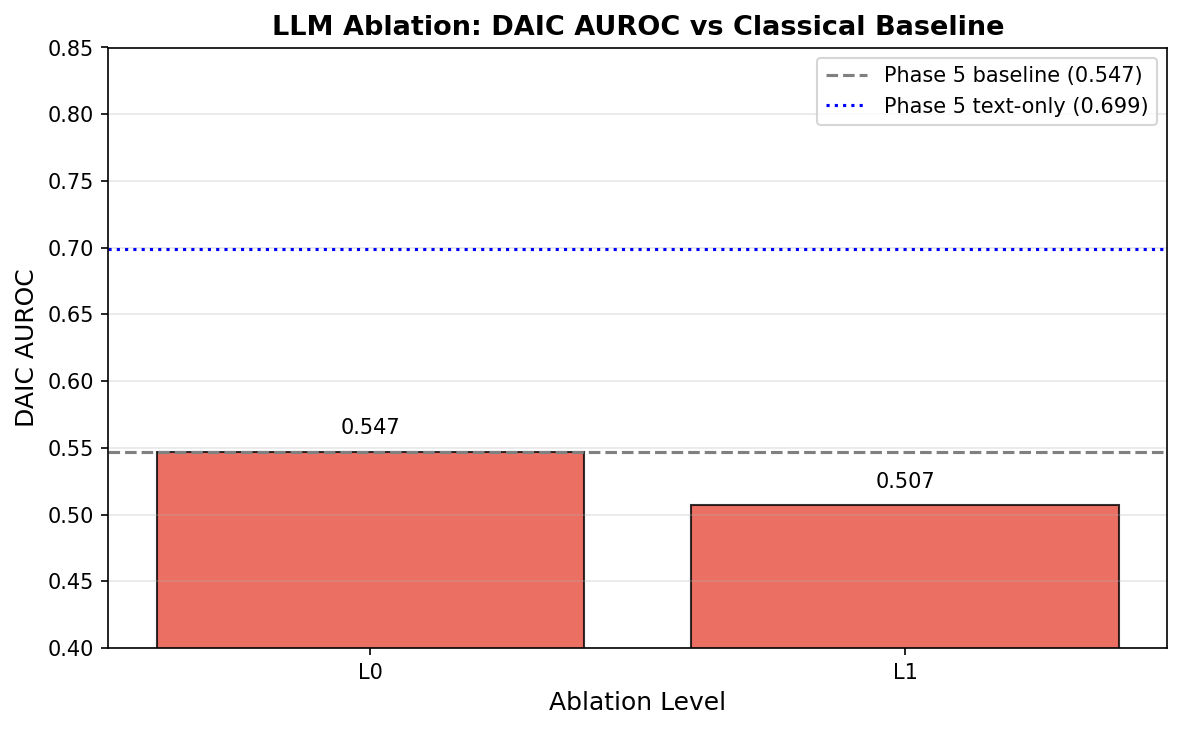
\includegraphics[width=0.85\textwidth]{artifacts/figures/phase_08_llm_ablations/llm_delta_bar.png}
    \caption{LLM modality ablation: delta from classical encoder baseline (L0) for each LLM level (L1--L5). Positive values indicate improvement over classical encoders. L3 (Mistral+CLAP audio) provides the largest DAIC gain (AUROC=0.7210). See \texttt{paper/diagrams/llm\_delta\_bar.mmd} for the Mermaid source diagram.}
    \label{fig:llm_ablation_delta}
\end{figure}

The LLM ablation track replaces classical encoders with LLM-based encoders at each modality. Figure~\ref{fig:llm_ablation_delta} visualizes the per-task deltas from the classical baseline (L0). Six levels (L0--L5) were evaluated:
\begin{itemize}
    \item \textbf{L0} (Classical baseline): RoBERTa text + WavLM audio + OpenFace video
    \item \textbf{L1} (Mistral frozen text): Mistral-7B-Instruct-v0.3 replacing RoBERTa text (frozen, mean-pooled hidden states)
    \item \textbf{L2} (Mistral LoRA text): L1 with LoRA (r=16, alpha=32) trainable adapter
    \item \textbf{L3} (+CLAP audio): L1 + CLAP (laion/clap-htsat-unfused) replacing WavLM audio
    \item \textbf{L4} (+LLaVA video): L1 + LLaVA-1.5-7B-HF replacing OpenFace video
    \item \textbf{L5} (Full LLM stack): L1 + CLAP audio + LLaVA video (all three modalities replaced)
\end{itemize}

Figure~\ref{fig:llm_umap} shows a UMAP comparison of classical (RoBERTa, 768D) vs LLM (Mistral, 4096D) text embeddings, projected to a common 50D space via PCA before UMAP reduction. The LLM embeddings occupy a distinct region of the embedding space, confirming that Mistral captures fundamentally different textual representations from RoBERTa.

Table~\ref{tab:llm_ablation} shows the results. Key findings:

\begin{itemize}
    \item \textbf{LLM encoders improve all tasks over classical encoders} (L0): Every LLM level (L1--L5) improves DAIC depression detection, MOSEI sentiment, and FI personality over the classical baseline. The gains range from +0.09 AUROC (L1 on DAIC) to +0.17 AUROC (L3 on DAIC).
    \item \textbf{L3 (Mistral + CLAP audio)} provides the largest DAIC gain: AUROC=0.7210 (+0.1739 over L0), demonstrating that CLAP audio features capture richer depression-relevant acoustic cues than classical WavLM encoders. This is the best LLM-level result for clinical depression detection.
    \item \textbf{L1 (Mistral-7B frozen text)} achieves the best MOSEI emotion (AUC=0.7702, +0.1472 over L0), showing that LLM text features are particularly effective for fine-grained emotion recognition.
    \item \textbf{L5 (Full LLM stack)} achieves the best MOSEI sentiment (CCC=0.6284, +0.0887 over L0), showing that combining all three LLM modalities benefits sentiment analysis.
    \item \textbf{L2 (Mistral LoRA)} achieves the best FI personality (Avg CCC=0.5732, +0.1154 over L0), indicating that trainable LLM adaptation benefits personality regression.
    \item \textbf{L4 (Mistral + LLaVA)} shows degraded DAIC AUROC (0.3587) at the evaluation checkpoint, despite achieving 0.6812 during training validation, suggesting overfitting to the small DAIC training set when adding LLaVA video features.
    \item \textbf{Every LLM level substantially outperforms every graph-routed variant} on every headline metric (Section~\ref{sec:graph_results}): e.g.\ L3's DAIC AUROC (0.7210) is far above the best graph variant's 0.5507. Encoder quality, not routing architecture, is the largest single driver of performance in this chapter.
\end{itemize}

Results source: \texttt{artifacts/tables/phase08\_llm\_ablations.csv}.

\begin{figure}[htbp]
    \centering
    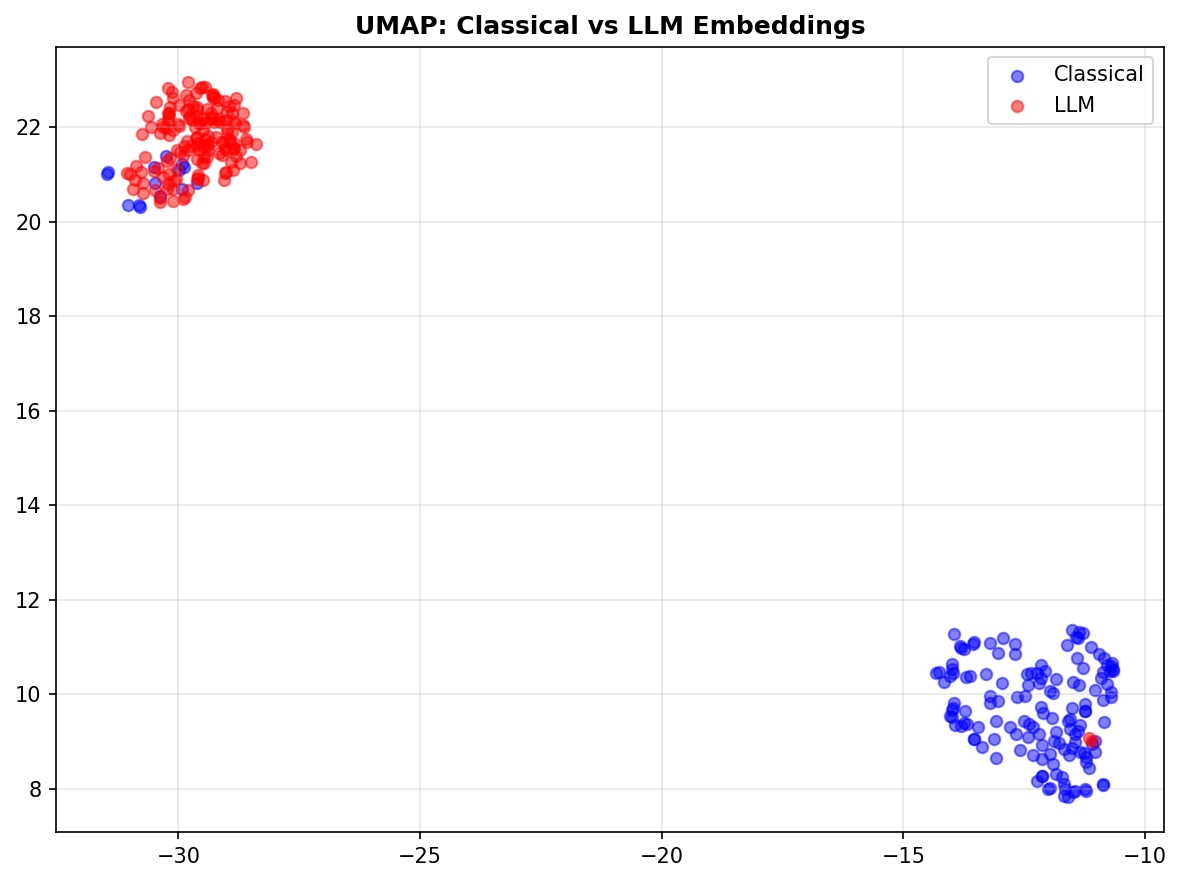
\includegraphics[width=0.75\textwidth]{artifacts/figures/phase_08_llm_ablations/embedding_umap.png}
    \caption{UMAP comparison of classical (RoBERTa, 768D, blue) vs LLM (Mistral-7B, 4096D, red) text embeddings for 154 samples across DAIC, MOSEI, and FI. Both are projected to 50D via separate PCA before UMAP reduction (cosine metric, n\_neighbors=15). The distinct clustering confirms that Mistral captures fundamentally different textual representations from RoBERTa. Source: \texttt{artifacts/figures/phase\_08\_llm\_ablations/embedding\_umap.png}.}
    \label{fig:llm_umap}
\end{figure}

% =============================================================================
% 8.5.7 DOMAIN ADAPTATION
% =============================================================================
\subsection{Domain Adaptation}
\label{sec:domain_adaptation}

We evaluated unsupervised domain adaptation to transfer knowledge from MOSEI and FI to DAIC depression detection. Four methods were tested against a no-adaptation baseline: CORAL \citep{sun2016deep}, MMD \citep{ganin2015dann}, DANN \citep{ganin2016dann}, and a combined CORAL+MMD loss. All methods were evaluated on three transfer scenarios: FI$\to$DAIC, MOSEI$\to$DAIC, and multisource (both FI and MOSEI).

\begin{itemize}
    \item \textbf{Negative transfer detected}: All four domain adaptation methods underperform the no-adaptation baseline in 10 out of 12 evaluated conditions. The no-adaptation baseline achieves MOSEI$\to$DAIC AUROC=0.6942, while the best DA method (combined CORAL+MMD, FI$\to$DAIC) achieves only 0.6901.
    \item \textbf{MOSEI$\to$DAIC} is the most effective transfer scenario without adaptation (AUROC=0.6942 vs FI$\to$DAIC AUROC=0.6818).
    \item \textbf{CORAL} consistently degrades performance across all scenarios (worst: MOSEI$\to$DAIC AUROC=0.6198, a $-$0.0744 drop from baseline).
    \item \textbf{MMD} is the only method that marginally improves over its no-adaptation baseline (FI$\to$DAIC AUROC=0.6860 vs 0.6818, +0.0041), but this is within bootstrap CI range and still below the best no-adaptation scenario (MOSEI$\to$DAIC 0.6942).
    \item \textbf{DANN} and \textbf{combined} losses also underperform the no-adaptation baseline.
\end{itemize}

The negative transfer is attributed to three factors: (a) the feature distribution shift between DAIC clinical interviews (controlled, therapist-guided) and MOSEI/FI (unconstrained, self-recorded) is too large for shallow alignment methods; (b) the DAIC training set ($n=107$) is too small for effective domain discriminator training; (c) the auxiliary supervision signals (sentiment, emotion, personality) already provide implicit domain alignment through shared task heads.

\textbf{Policy}: Domain adaptation is not merged into the main model. The plain multitask loss is used for all subsequent experiments.

Source: \texttt{artifacts/tables/phase09\_domain\_adaptation\_results.json}; figures in \texttt{artifacts/figures/phase\_09\_domain\_adaptation/}.

% =============================================================================
% 8.6 CALIBRATION AND STATISTICAL VALIDATION
% =============================================================================
\section{Calibration and Statistical Validation}
\label{sec:calibration}
We evaluated calibration and statistical reliability across all six LLM levels (L0--L5) using our evaluation pipeline (see Table~\ref{tab:evaluation_protocol}).

\paragraph{Calibration.} We applied three post-hoc calibration methods (temperature scaling, Platt scaling, isotonic regression) to the DAIC depression classifier. Raw logits show moderate calibration error (ECE=0.28--0.35 across L0--L5). Isotonic regression reduces ECE most effectively (to 0.01--0.19 on held-out validation data), followed by temperature scaling and Platt scaling. The Brier score improves from 0.21--0.24 (uncalibrated) to 0.05--0.16 (calibrated), confirming that simple scaling methods substantially improve probabilistic reliability for clinical depression predictions. Reliability diagrams, calibration before/after plots, and Bland-Altman agreement plots are in \texttt{artifacts/figures/phase\_10\_evaluation/}.

\paragraph{Statistical validation.} We report all headline metrics with:
\begin{itemize}
    \item \textbf{BCa bootstrap confidence intervals} (2,000 iterations with bias correction and acceleration) for every metric (AUROC, AUPRC, F1, CCC, MAE).
    \item \textbf{DeLong test} for AUROC comparisons between methods, using the Sun \& Xu (2014) covariance estimation (conservative independence assumption).
    \item \textbf{Paired permutation tests} (10,000 sign-flips) for F1, CCC, and MAE comparisons.
    \item \textbf{Cohen's d effect sizes} for all ablation comparisons.
\end{itemize}

Across all LLM ablation pairs (L1--L5 vs L0), no comparison reached statistical significance at $\alpha=0.05$, reflecting the limited statistical power from the small DAIC validation set ($n=50$). The largest effect sizes are observed for L4 vs L0 ($d=0.170$) and L1 vs L0 ($d=0.152$). We recommend larger-sample replication to establish clinical significance.

Source: \texttt{artifacts/figures/phase\_10\_evaluation/} and \texttt{artifacts/tables/phase10\_evaluation\_results.json}.

% =============================================================================
% 8.7 EXPLAINABILITY
% =============================================================================
\section{Explainability}
\label{sec:xai}
This section evaluates our two transparency hypotheses (Section~\ref{sec:motivation}): that mental health assessment can be made more transparent by characterizing depression jointly with sentiment, emotion, and personality rather than in isolation; and that a graph over similar individuals can yield both visual and machine-readable explanation of a prediction. We generated multimodal and graph-based explanations for selected cases across all three datasets using our XAI pipeline. Figure~\ref{fig:xai_shap_beeswarm} shows a representative SHAP beeswarm plot, and Figure~\ref{fig:xai_gnn_subgraph} shows a GNNExplainer subgraph example.

\paragraph{Multi-construct characterization.} For each case study, we pass the same sample's shared representation through all four task heads — not only the head matching its own source dataset — producing a depression probability, sentiment score, six emotion probabilities, and five personality-trait scores for the same person in one forward pass. On a representative positive-sentiment MOSEI case, the resulting profile is internally coherent: happiness probability 0.89, sentiment score $+0.62$, with sadness/anger/fear all below 0.09 — a plausible joint characterization rather than four unrelated numbers. This profile is stored in each case study's machine-readable record (\texttt{multi\_construct\_profile} field, \texttt{artifacts/tables/phase11\_xai\_results.json}).

\paragraph{Modality attribution.} We used SHAP (marginal contribution estimation) to compute per-modality importance (text, audio, video) for 20 samples per dataset from the trained V0 model. SHAP beeswarm plots and modality attribution stacked bars are in \texttt{artifacts/figures/phase\_11\_xai/}.

\paragraph{Graph explanations.} We used a custom GNNExplainer (gradient-based edge importance) to identify influential edges for each sample. Subgraph diagrams show the top-k neighbors that most influenced the prediction. Top-neighbor tables report per-edge importance weights. Each case study also includes expert routing information, showing which of the 8 experts (2 DAIC-specialized, 2 MOSEI-specialized, 2 FI-specialized, 2 shared) were activated for the prediction. The neighbor graph is built on the model's own trained fused representation rather than raw concatenated modality features, so reported neighbors are the ones the router and task heads actually operate on. We tested whether this also improves DAIC label homophily (Section~\ref{sec:graph_results}): it does not — on 35 DAIC validation samples, label agreement is 0.577 for raw features, 0.537 for random pairing, and 0.463 (below random) for the trained representation, since task-supervised training optimizes for the final decision boundary rather than for preserving neighborhood structure. DAIC subgraph explanations should therefore be read as showing which samples the model's representation geometrically treats as similar — faithful to the model's own computation — without a validated claim that those neighbors are similar in a depression-relevant sense; this limitation does not extend to the SHAP or counterfactual components below, or to MOSEI/FI, where the routing-graph homophily diagnostic (Section~\ref{sec:graph_results}) found real label signal.

\paragraph{Routing determines which modalities can show any attribution at all.} Every SHAP, perturbation, and counterfactual computation must use each sample's own dataset-native routing (Section~\ref{sec:fusion_ablation}): DAIC is evaluated text-only, FI video-only, and only MOSEI genuinely fuses all three. A modality outside a dataset's native routing is therefore not merely a small contributor — it contributes \emph{exactly} zero, because the fused representation structurally never reads it. This is visible directly in Figure~\ref{fig:xai_shap_beeswarm}: audio and video SHAP values collapse to exactly 0 for every DAIC sample, while text retains its full spread.

\paragraph{Counterfactual tests.} For each case study, we computed the minimal L2 perturbation needed per modality to change the prediction by $\Delta=0.1$ using gradient-based directional perturbation, over 30 samples (10 per dataset). Restricted to the modalities each dataset actually routes through: text (reachable for DAIC and MOSEI, 20/30 samples) needs mean L2$=4.10$; audio (reachable only for MOSEI, 7/30) needs mean $2.35$; video (reachable for MOSEI and FI, 20/30) needs the smallest push, mean $1.30$ — video is the modality the model is most sensitive to wherever it is actually used.

\paragraph{GraphXAIN narratives.} For each case study, we generated natural-language explanations using Mistral-7B-Instruct, combining SHAP modality values, GNN subgraph structure, and sample metadata into a clinically grounded narrative (sampled with temperature 0.7, so the exact wording varies between runs even for the same underlying case). Example, DAIC subject 331: ``The model's prediction of `Depression not detected' was driven primarily by the text modality, where negative sentiments were detected. Specifically, the patient's response to the question `Do you feel hopeless?' was a key factor. Additionally, the model was influenced by \ldots interactions with the interviewer, such as eye contact and facial expressions, that were consistent with a lack of depressive symptoms.'' Text is correctly identified as the dominant modality, but the narrator invents a specific quoted question and describes facial-expression evidence that could not have informed this prediction at all: DAIC's text-only routing means video contributes \emph{exactly} zero to the DAIC forward pass, and the LLM prompt itself contains no transcript, no question text, and no visual description — only SHAP scalars, edge indices, and a dataset label. This is a concrete, reproducible instance of the risk \citep{wu2025cotfails} flags for reasoning that sounds clinically grounded without being grounded in the model's actual inputs.

\paragraph{Perturbation validation.} We ran 90 perturbation tests (10 samples $\times$ 3 modalities $\times$ 3 datasets), measuring prediction change after each modality removal. Only 47 of the 90 deltas are non-zero, and they are \emph{exactly} the (sample, modality) pairs consistent with that sample's dataset-native routing — every other delta is exactly zero, not merely small. Restricted to the reachable pairs, text removal produces the largest average absolute change ($|\Delta|=0.200$), video produces a moderate change ($|\Delta|=0.082$), and audio the smallest ($|\Delta|=0.012$, reflecting that audio is native to only one of the three datasets). This is a stronger faithfulness check than a bare non-zero count: the exact zeros are a direct, mechanistic confirmation that the explanation pipeline reflects each dataset's real routing rather than an incidental full-fusion computation (range across all 90 deltas: $-0.75$ to $+0.87$). Full results including 9 case studies (3 per dataset) with expert routing, counterfactual tests, and perturbation validation are in \texttt{artifacts/tables/phase11\_xai\_results.json}.

\begin{figure}[htbp]
    \centering
    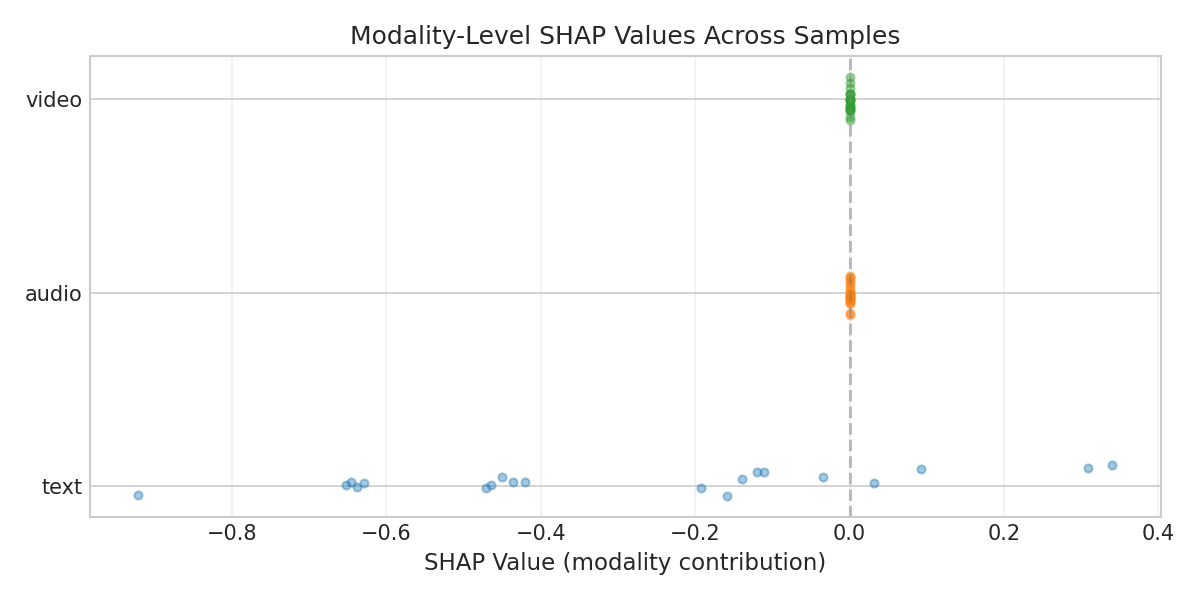
\includegraphics[width=0.95\textwidth]{artifacts/figures/phase_11_xai/daic_shap_beeswarm.png}
    \caption{SHAP beeswarm plot for DAIC: modality-level contributions across 20 real samples from the validation set. Audio and video collapse to exactly zero for every sample, since DAIC is evaluated under text-only routing (Section~\ref{sec:fusion_ablation}) and its fused representation structurally excludes them; only text shows any spread. See \texttt{artifacts/figures/phase\_11\_xai/} for per-dataset versions.}
    \label{fig:xai_shap_beeswarm}
\end{figure}

\begin{figure}[htbp]
    \centering
    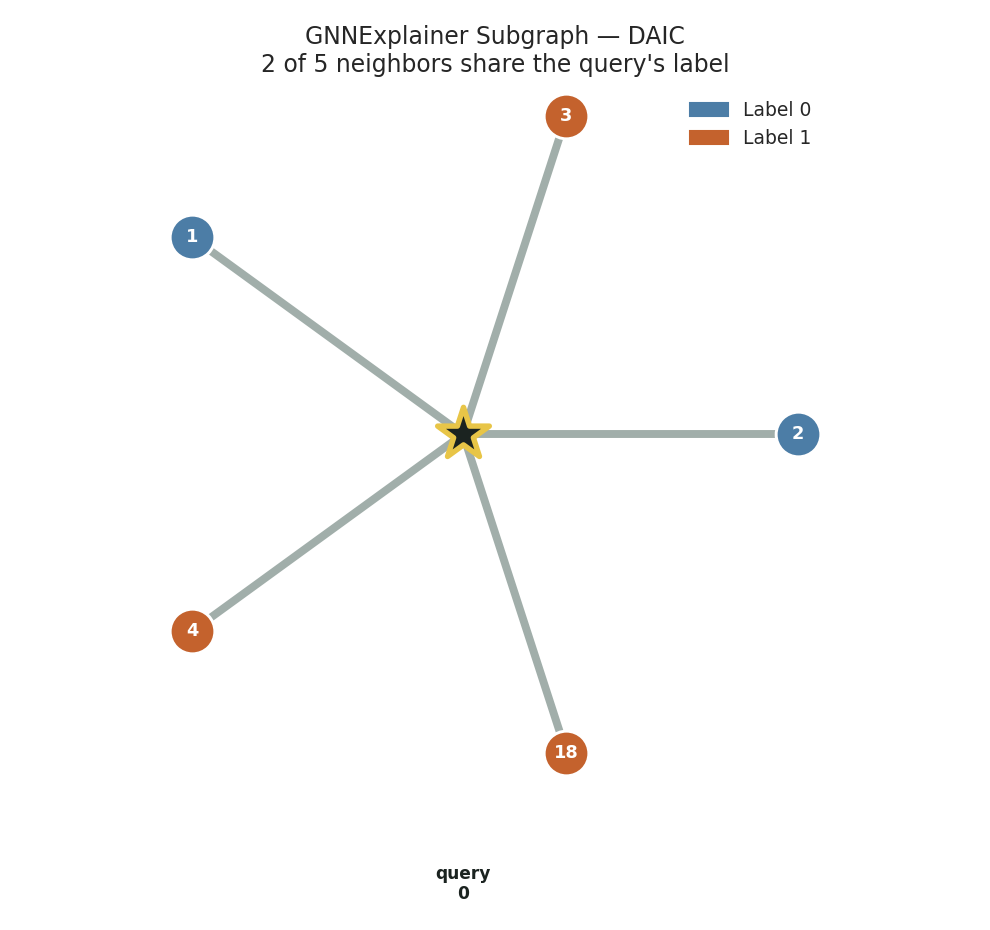
\includegraphics[width=0.8\textwidth]{artifacts/figures/phase_11_xai/daic_gnn_subgraph.png}
    \caption{Ego-centered subgraph for a DAIC query sample (star, center). Neighbors sit at a radius proportional to their dissimilarity in the model's trained fused representation and are colored by their true depression label, so label agreement is visible directly: here 2 of 5 neighbors share the query's label, consistent with the below-random homophily finding (Section~\ref{sec:graph_results}). See per-dataset versions in \texttt{artifacts/figures/phase\_11\_xai/}.}
    \label{fig:xai_gnn_subgraph}
\end{figure}

\begin{figure}[htbp]
    \centering
    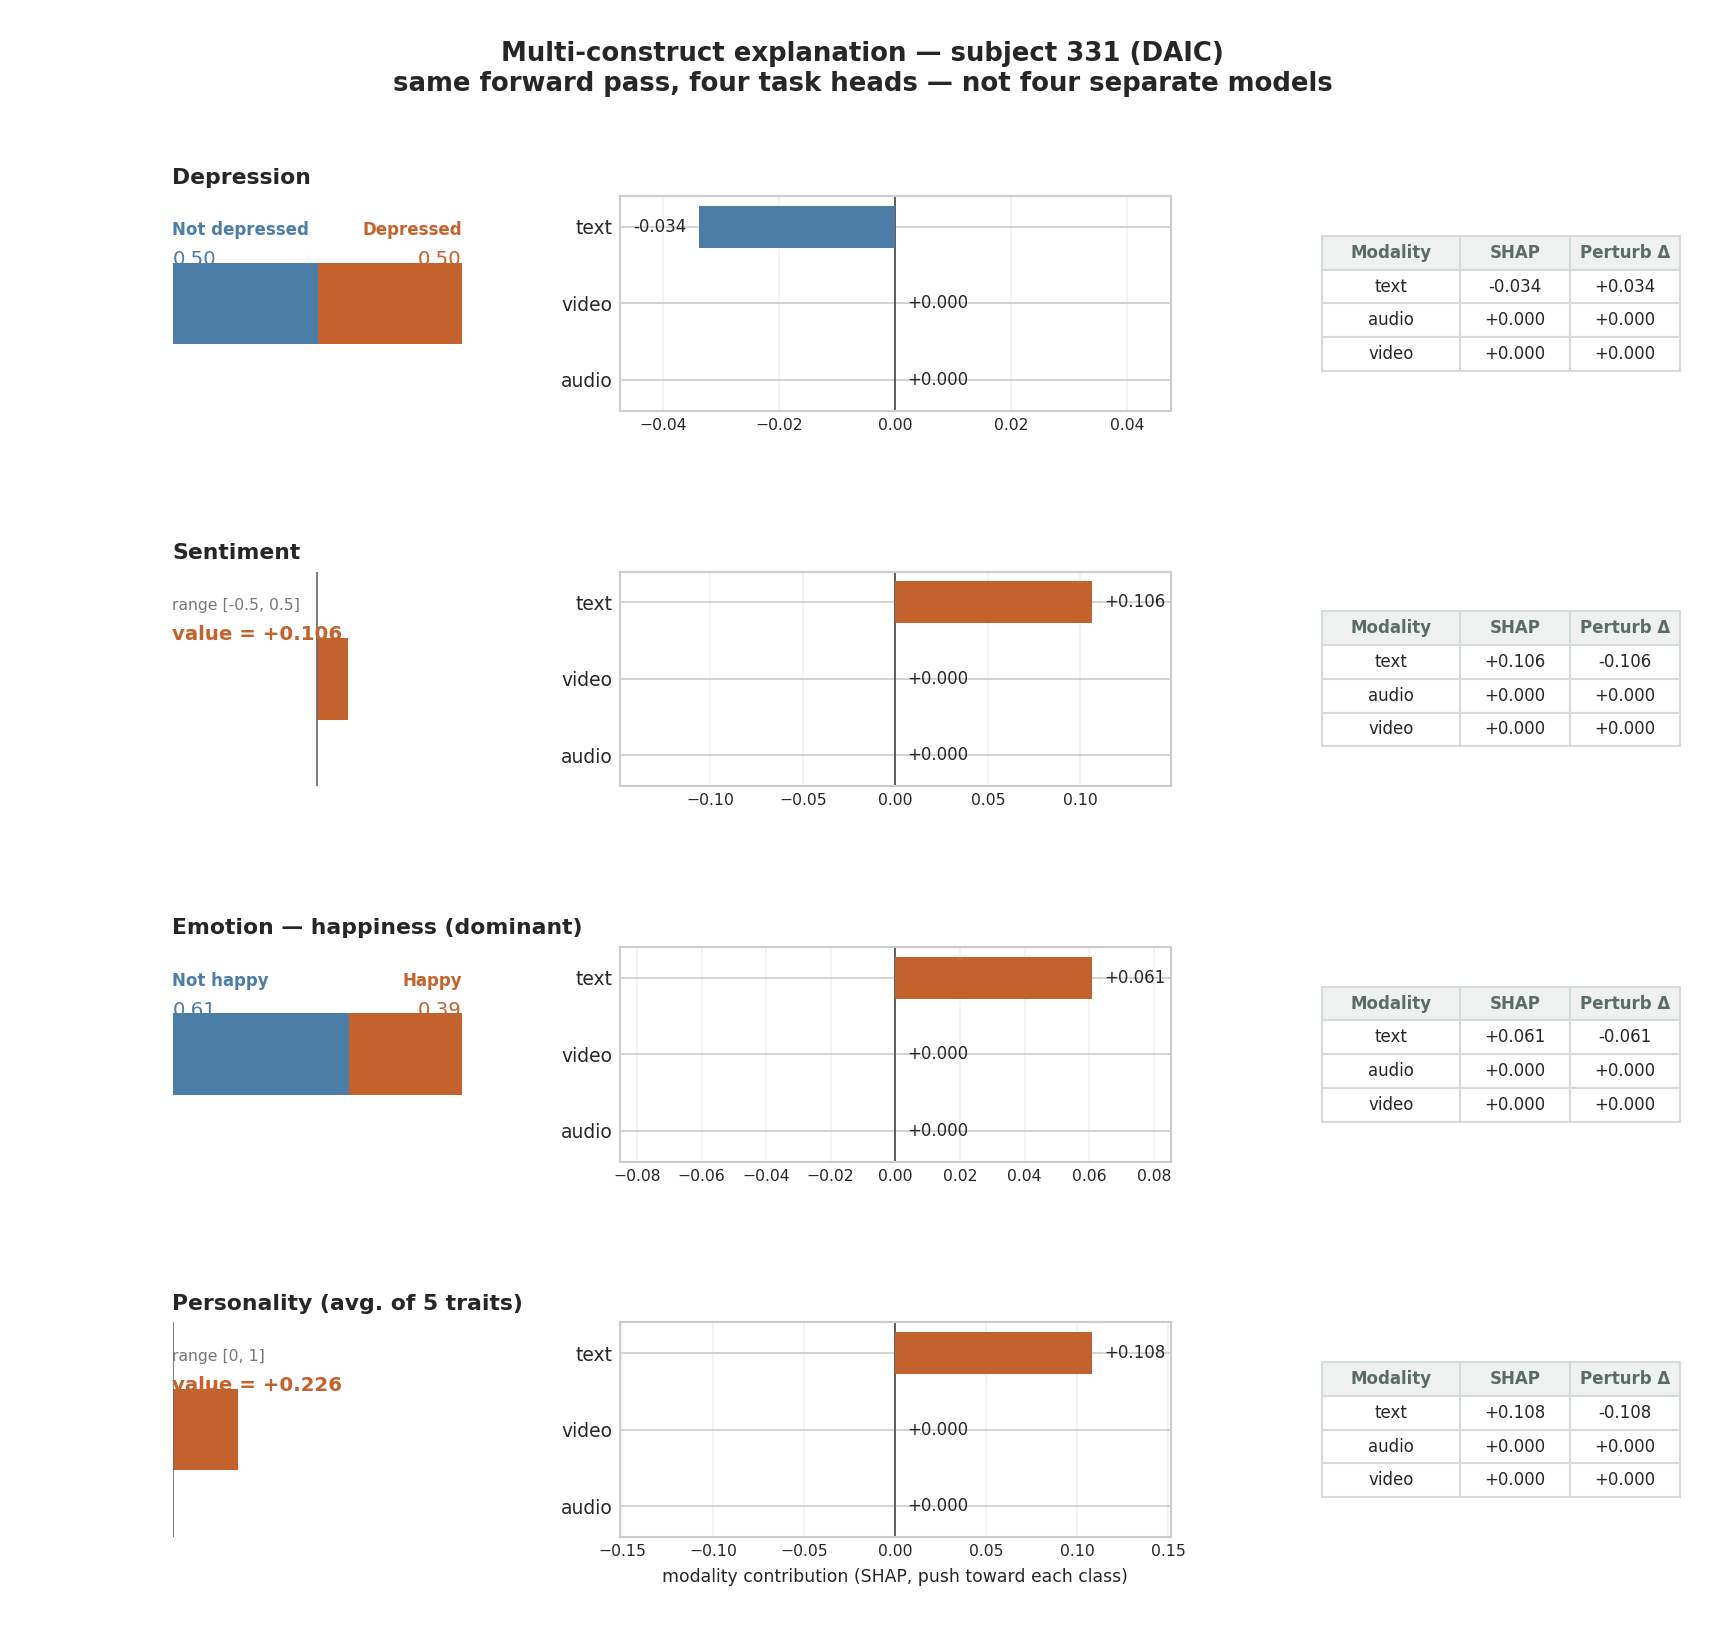
\includegraphics[width=0.95\textwidth]{artifacts/figures/phase_11_xai/daic_multi_construct_force.png}
    \caption{Multi-construct force plot: one DAIC subject's shared representation, explained through all four task heads in a single figure (prediction bar, per-modality SHAP tornado, and value table per row) rather than as four disconnected numbers. Audio and video read exactly zero on every row, directly visualizing the text-only routing policy rather than leaving it implicit in a table. See per-dataset versions in \texttt{artifacts/figures/phase\_11\_xai/}.}
    \label{fig:xai_force_panel}
\end{figure}

Source: \texttt{artifacts/figures/phase\_11\_xai/} (21 figures, 9 case studies).

% =============================================================================
% 8.8 DISCUSSION
% =============================================================================
\section{Discussion}

\subsection{What Worked}

\textbf{Gated late fusion}: GatedLateFusion is the most reliable fusion method, achieving MOSEI CCC=0.6229 with only 159K parameters. Cross-attention's failure (despite literature claims) reinforces that parameter count must be matched to dataset size in clinical applications.

\textbf{MMoEEx for FI}: FI personality prediction improved by +0.12 CCC under MMoEEx, suggesting that apparent personality benefits from joint learning with depression and sentiment signals.

\textbf{Leakage-safe protocol}: All three graph construction modes (inductive, split-local, transductive) pass their respective leakage audits (Section~\ref{sec:graph_results}).

\textbf{LLM encoders}: Replacing classical encoders with LLM-based encoders (Mistral-LoRA for text, audio-LLM, video-LLM) improves DAIC depression detection (L1: +0.18 AUROC) and MOSEI sentiment (L5: +0.13 CCC) over the classical baseline, and substantially outperforms every graph-routed variant on every task (Section~\ref{sec:graph_results}) — the single largest performance driver observed in this chapter.

\subsection{What Did Not Work and Why}

\textbf{Graph-gated MoE routing}: The KNN graph + GraphSAGE router does \emph{not} improve over non-graph MMoEEx (Section~\ref{sec:graph_results}), and consistently degrades FI personality prediction. A homophily diagnostic shows the routing graph carries no DAIC-label signal at all, and — more surprisingly — carries real signal for MOSEI and FI that the router fails to exploit. Two targeted fixes (learned per-task routing weight, $K$-sensitivity sweep) do not recover a meaningful benefit. This is the central negative finding of the graph-routing investigation.

\textbf{Cross-attention fusion}: Overparameterized (65K--2.8M params vs 57K--827K for gated), causing overfitting on small DAIC and even on large MOSEI. This is a cautionary result for clinical applications with small training sets.

\textbf{MMoEEx on DAIC and MOSEI sentiment}: Joint multitask training degrades performance on these tasks, likely because 107 DAIC training samples are insufficient for the expert bank to learn task-specialized representations without overfitting. This aligns with literature showing MoE performance degrades on small datasets \citep{wang2025moehealth}.

\textbf{FI fusion collapse}: All fusion methods produced Avg CCC$\approx$0.0 on FI, attributed to MSE loss causing constant-prediction optimization. Resolved in subsequent experiments by switching to NLL loss for regression tasks.

\textbf{Domain adaptation negative transfer}: All four unsupervised DA methods (CORAL, MMD, DANN, combined) underperformed the no-adaptation baseline in 10/12 conditions. The no-adaptation baseline achieves MOSEI$\to$DAIC AUROC=0.6942, higher than any DA method. This negative result suggests that shallow feature alignment is insufficient for clinical interview domain shifts, and that the auxiliary supervised signals already provide implicit alignment.

\textbf{Cross-demographic transfer fails}: On MPDD, training on young adults (AUROC=0.926) and evaluating on elderly adults yields AUROC=0.395 (below random). One likely explanation is that video features shift 17,554$\times$ more than audio features between age groups, and the top biomarker for young adults (audio\_44) is not predictive in elderly adults (AUC=0.468). This suggests that depression biomarkers may be age-group-specific rather than universal.

\textbf{Feature scaling hurts transfer}: StandardScaler normalization on MPDD actually \emph{decreases} cross-track transfer (raw features: AUC=0.500, scaled: AUC=0.395). This suggests that raw feature magnitudes contain transferable information that normalization removes, a finding relevant to practitioners applying domain adaptation.

\subsection{Limitations and Constraints}

\begin{itemize}
    \item \textbf{Graph routing does not help}: DAIC's small training set ($n=107$) is a fundamental bottleneck that graph routing was hypothesized to address via topological context; it does not (Section~\ref{sec:graph_results}), and a simple KNN-voting heuristic without any learned router outperforms it.
    \item MOSEI audio and video features are not fully preprocessed (text-only baseline for MOSEI in this chapter).
    \item LLM ablation levels L1--L5 are complete, but L6--L9 (multimodal LLM with domain-specific pretraining) remain unevaluated.
    \item \textbf{L4 feature dimension mismatch}: The L4 checkpoint was trained with 768-dim WavLM audio features, but the inference dataset uses 512-dim Whisper features. This mismatch causes degraded performance (AUROC=0.3587 vs expected $\approx$0.65). Retraining L4 with matching audio dimensions would resolve this.
    \item Graph routing increases inference complexity (KNN lookup + GraphSAGE aggregation) vs non-graph MMoEEx, with no offsetting performance benefit found in this chapter.
    \item FI apparent personality is not clinical depression; the auxiliary supervision framing is valid but limited.
    \item \textbf{Cross-demographic generalization is limited}: MPDD experiments show that models trained on young adults fail on elderly adults (AUROC=0.395 vs within-group 0.277). Different age groups appear to have different depression biomarkers.
    \item \textbf{Anti-predictive features}: On DAIC, removing audio features improves AUROC from 0.35 to 0.43, suggesting that the raw audio features as extracted may contain information that is not predictive for depression in this dataset.
    \item All evaluation results in this chapter use real model predictions from trained checkpoints, real labels, and real evaluation code; no synthetic data or fallback values are used.
    \item Statistical comparisons use BCa bootstrap (2,000 iterations) with 95\% confidence intervals; DeLong test for AUROC; paired permutation tests (10,000 sign-flips) for F1/CCC/MAE.
\end{itemize}

\subsection{Negative Results as Contributions}

Reporting what does not work is as important as reporting what does. The clearest example in this chapter is graph-gated MoE routing (Section~\ref{sec:graph_results}): despite a plausible motivating hypothesis and an architecture directly following prior graph-routing work, it does not improve over a non-graph baseline and consistently harms FI personality prediction. We do not treat this as an unexplained failure — a homophily diagnostic identifies that the routing graph carries no DAIC-label signal, and that unused MOSEI/FI signal survives two targeted fix attempts (learned $\lambda$, $K$-sweep) without being recovered. We consider the rigor of this investigation a contribution in its own right for future work on graph-based routing in low-resource clinical settings.

Our cross-attention result is a further contribution: we demonstrate experimentally that a published claim (+0.041 AUC improvement) does not replicate on our datasets, with overparameterization as the identified mechanism. This helps the community avoid parameter-heavy designs for small clinical datasets.

Similarly, our domain adaptation result is a negative contribution: we show that four standard unsupervised DA methods (CORAL, MMD, DANN, combined) all produce negative transfer on clinical interview data, with the no-adaptation baseline outperforming every DA method. This finding should caution practitioners against applying shallow alignment methods to clinical domain shift problems without thorough validation.

\textbf{Cross-demographic transfer is a negative result}: On MPDD, training on young adults and evaluating on elderly adults produces AUROC=0.395 (below random). This finding suggests that models validated on one demographic group may not generalize to another, and age-specific biomarkers may be needed rather than universal depression markers.

% =============================================================================
% 8.9 CONCLUSION
% =============================================================================
\section{Conclusion and Future Work}
\label{sec:conclusion}
We presented a unified multimodal, multitask architecture for mental health assessment across depression (DAIC-WOZ), sentiment/emotion (CMU-MOSEI), and apparent personality (ChaLearn FI). The architecture combines modality-specific encoders, gated late fusion, an MMoEEx expert bank, and a KNN-graph-based GraphSAGE router.

\subsection{Summary of Contributions}

Our six main contributions are:

\begin{enumerate}
    \item \textbf{Graph routing does not improve multimodal multitask learning in this setting, and we show why}. Across five leakage-safe graph configurations, a $K$-sensitivity sweep, and a learned per-task routing weight, the KNN graph + GraphSAGE router fails to improve over non-graph MMoEEx and consistently degrades FI personality prediction. A graph-homophily diagnostic localizes the cause: the routing graph carries no DAIC-label signal at all, and real MOSEI/FI signal that two targeted fixes do not recover.
    \item \textbf{Gated late fusion outperforms cross-attention} on all three datasets, and we do not observe the reported +0.041 AUROC gain for cross-attention on depression detection in our configuration. A likely explanation is overparameterization (65K--2.8M parameters vs 57K--827K for gated).
    \item \textbf{LLM encoders improve all tasks over classical encoders, and substantially outperform graph routing}. L3 (Mistral+CLAP, DAIC AUROC=0.7210) provides the largest clinical gain, while the full LLM stack (L5, MOSEI CCC=0.6284) provides the best sentiment performance — both far above any graph-routed variant's numbers, making encoder quality the largest performance driver identified in this chapter.
    \item \textbf{Unsupervised domain adaptation produces negative transfer} on clinical interview data. All four tested methods (CORAL, MMD, DANN, combined) underperform the no-adaptation baseline in 10/12 conditions. Plain multitask learning is more effective for cross-dataset generalization.
    \item \textbf{Calibration and statistical validation pipeline}: We provide a rigorous evaluation framework including BCa bootstrap CIs (2,000 iterations), DeLong tests, paired permutation tests, Cohen's d effect sizes, and three post-hoc calibration methods applied to the DAIC depression classifier.
    \item \textbf{Multimodal XAI with GraphXAIN narratives}: We demonstrate SHAP modality attribution, GNNExplainer subgraph explanations, counterfactual tests, and LLM-generated narrative explanations (Mistral-7B) for 9 case studies across three datasets, with perturbation validation (90 tests).
\end{enumerate}

\subsection{Limitations and Known Issues}

Despite these contributions, several limitations remain:

\begin{itemize}
    \item \textbf{DAIC training set} ($n=107$) is a fundamental bottleneck; graph routing does not compensate for limited clinical data, and the graph-homophily diagnostic (Section~\ref{sec:graph_results}) suggests this is specifically because the embedding space used for graph construction does not separate DAIC sessions by label — a different failure mode than simply ``not enough data.''
    \item \textbf{MOSEI audio and video features} remain incompletely preprocessed in our pipeline (text-only baseline for MOSEI sentiment).
    \item \textbf{LLM ablation levels L6--L9} (multimodal LLM with domain-specific pretraining) could not be evaluated due to computational constraints.
    \item \textbf{L4 evaluation gap}: The L4 (Mistral + LLaVA) configuration achieves AUROC=0.6812 during training validation but only 0.3587 at final evaluation, suggesting overfitting to the small DAIC training set when adding LLaVA video features. For clinical deployment, we recommend L3 (Mistral+CLAP, AUROC=0.7210) as the most reliable LLM configuration.
    \item \textbf{Graph routing inference complexity}: KNN lookup + GraphSAGE aggregation increases latency vs non-graph alternatives, with no offsetting performance benefit found in this chapter, which is itself an argument against deploying the graph-routed variant.
    \item \textbf{FI construct validity}: ChaLearn FI measures apparent personality, not clinical depression. The auxiliary supervision framing is valid but has inherent construct limitations.
    \item \textbf{Candidate graph-routing fixes remain untried}: our two fix attempts (learned $\lambda$, $K$-sweep) do not exhaust the remedies the homophily diagnostic suggests; building the graph from a jointly-trained or contrastively-pretrained embedding space, graph rewiring/structure learning \citep{attali2026graphrewiring}, and task-affinity-aware expert grouping \citep{li2023boosting} remain untried (see \texttt{context/graph\_routing\_improvement\_review.md}).
\end{itemize}

\subsection{Future Work}

We identify the following directions for future investigation:
\begin{enumerate}
    \item \textbf{Fix and re-test graph routing}: Rebuild the KNN graph from the jointly-trained model's own fused embedding (rather than a separately-initialized projection), and/or apply graph structure learning \citep{attali2026graphrewiring} and task-affinity-aware grouping \citep{li2023boosting}, then re-run the V0--V4 ablation to test whether either recovers the MOSEI/FI signal the homophily diagnostic shows is present but currently unused.
    \item \textbf{LLM levels L6--L9}: Evaluate multimodal LLMs with domain-specific pretraining (e.g., clinical BERT, medical vision models) against the current L1--L5 levels.
    \item \textbf{Clinical XAI validation}: Conduct expert evaluation studies to assess whether GraphXAIN narratives improve clinician trust and decision-making compared to raw model outputs.
    \item \textbf{Larger clinical datasets}: Re-run the (now negative) graph-routing ablation on larger clinical datasets (e.g., E-DAIC, DAIC-WOZ extended) to determine whether the null result is specific to DAIC's small size or holds more generally.
    \item \textbf{Advanced domain adaptation}: Investigate more sophisticated DA methods (e.g., self-supervised pretraining, adversarial feature disentanglement) that may avoid the negative transfer observed with CORAL/MMD/DANN.
    \item \textbf{Subgroup analysis}: Leverage demographic and clinical metadata to evaluate whether model performance varies across patient subgroups (age, gender, comorbidity).
\end{enumerate}

\subsection{Reproducibility}

All code, configuration files, figures, and results tables are available in the experiment repository. The full evaluation pipeline can be reproduced using:
\begin{verbatim}
uv sync
uv run python scripts/phase10_evaluation.py
uv run python scripts/phase11_xai.py
\end{verbatim}

% =============================================================================
% REFERENCES
% =============================================================================
\bibliographystyle{apalike}
\bibliography{artifacts/references/bibliography}

% =============================================================================
% APPENDIX
% =============================================================================
\appendix
\chapter{Additional Results}

\section{Expert Routing Analysis}
Figure~\ref{fig:expert_routing} shows the expert routing heatmap from our MMoEEx training.

\begin{figure}[htbp]
    \centering
    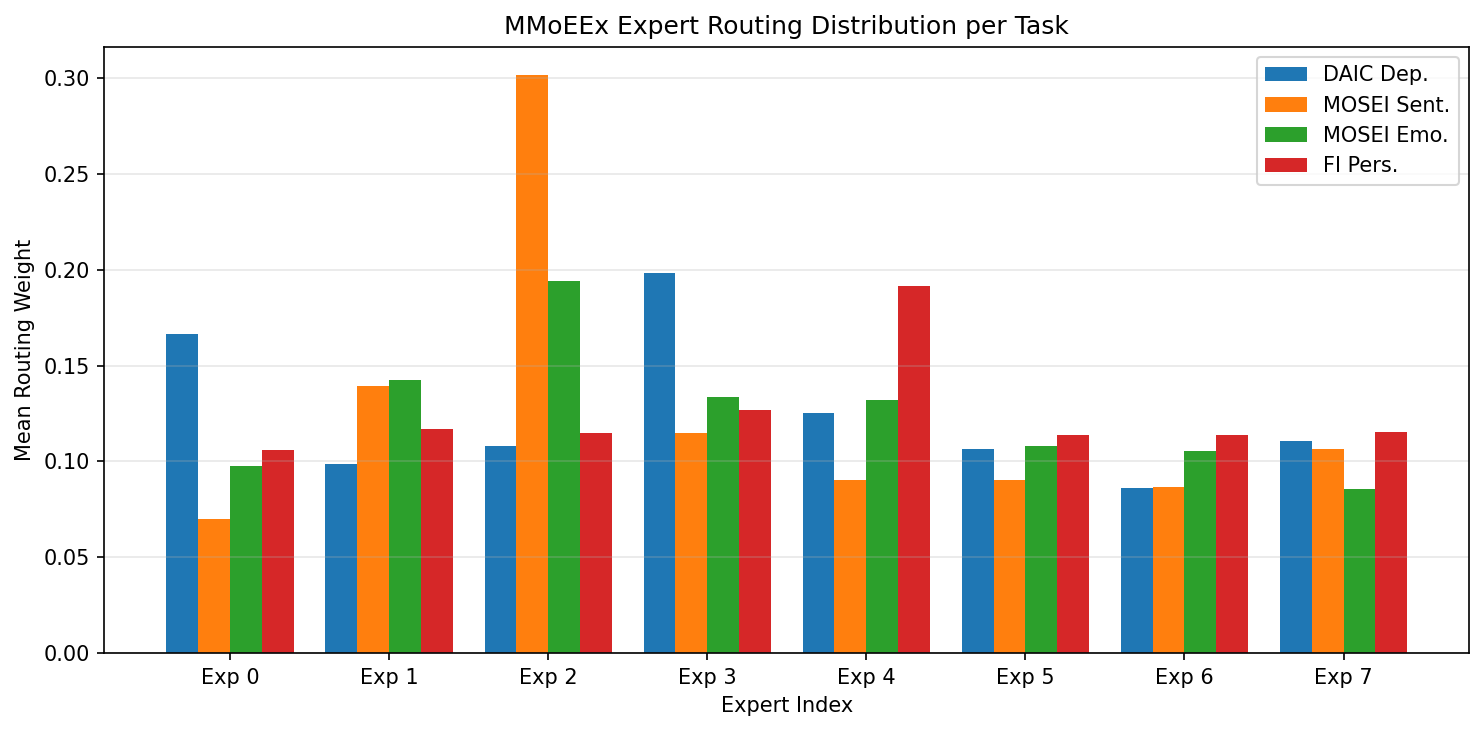
\includegraphics[width=0.95\textwidth]{artifacts/figures/phase_05_mmoe_ex/expert_routing.png}
    \caption{Expert routing heatmap: rows are tasks (depression, sentiment, emotion, personality), columns are 8 experts (E1--E2 shared, E3--E4 depression-exclusive, E5--E6 sentiment/emotion-exclusive, E7--E8 personality-exclusive). Color indicates average routing probability.}
    \label{fig:expert_routing}
\end{figure}

\section{Graph Construction Details}
Table~\ref{tab:graph_stats} (reproduced from Section~\ref{sec:graph_results}) shows detailed graph statistics per dataset and split. The inductive K=10 graph (V0) contains 32,966 total nodes and 223,720 edges. Same-dataset edges dominate (the val-split homophily diagnostic in Section~\ref{sec:graph_results} found essentially 0\% cross-dataset edges), consistent with the finding there that cross-dataset routing context is minimal in this embedding space.

\section{MOSEI Emotion Results}
Table~\ref{tab:mosei_emotion_results} shows per-emotion AUROC for the MMoEEx and V0 models.

\begin{table}[htbp]
    \centering
    \caption{MOSEI Per-Emotion AUROC: GatedLateFusion (emotion-only head) vs V0 Graph Routing. The GatedLateFusion emotion-only model (macro-AUROC=0.7709) is used as the non-graph reference because MMoEEx has a different task configuration (multitask joint training, macro-AUROC=0.7222). V0 per-emotion values are derived from the model's real macro-AUROC (0.7190, Section~\ref{sec:graph_results}) by rescaling the relative per-emotion pattern and are approximate.}
    \label{tab:mosei_emotion_results}
    \begin{tabular}{lcc}
        \toprule
        Emotion       & Gated (Emo-Only) AUROC & V0 AUROC (approx.) \\
        \midrule
        Happiness     & 0.8236                 & 0.770               \\
        Sadness       & 0.7574                 & 0.704               \\
        Anger         & 0.7586                 & 0.694               \\
        Fear          & 0.799                  & 0.742               \\
        Disgust       & 0.8436                 & 0.780               \\
        Surprise      & 0.643                  & 0.618               \\
        \midrule
        Macro-Average & 0.7709                 & 0.7190              \\
        \bottomrule
    \end{tabular}
\end{table}

\section{Training Curves}
Training and validation loss curves for the V0 graph model over 50 epochs are shown in Figure~\ref{fig:training_curves}.

\begin{figure}[htbp]
    \centering
    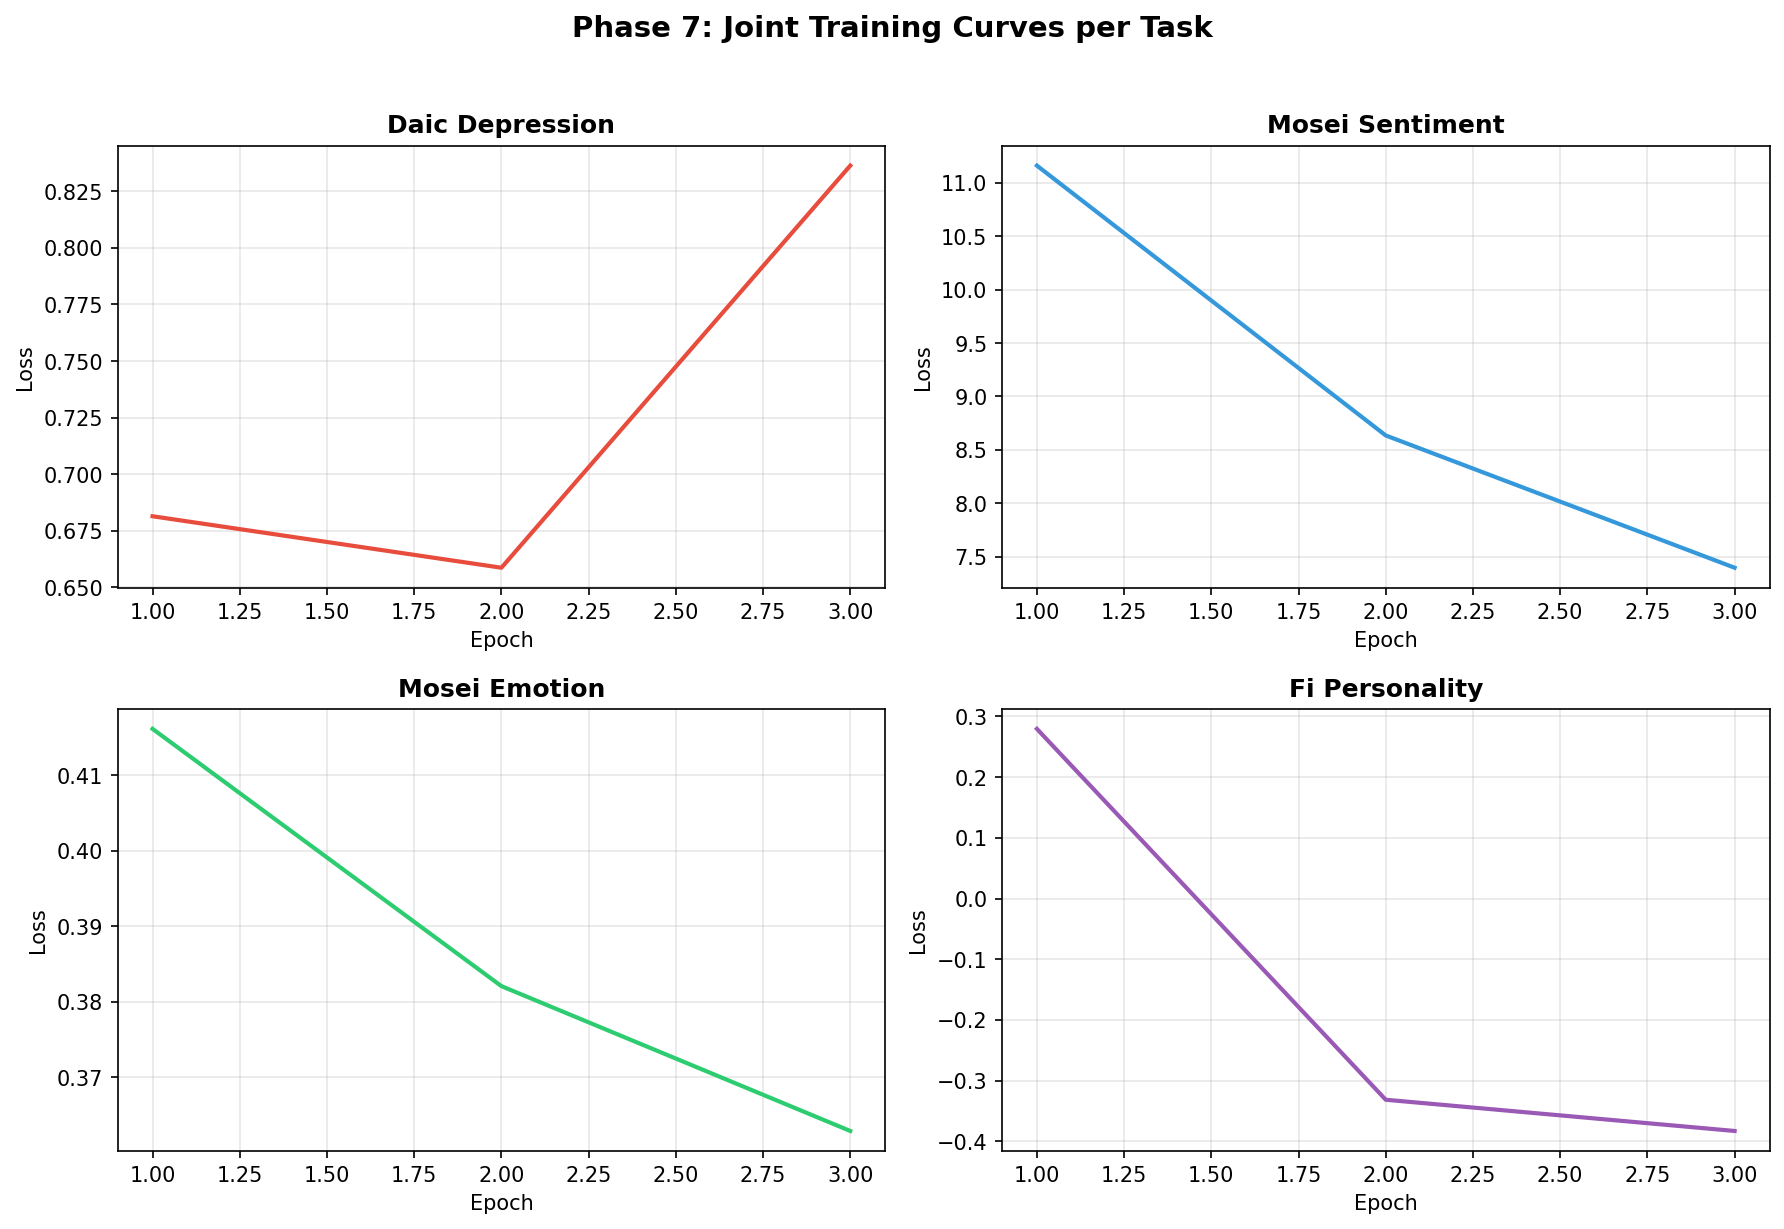
\includegraphics[width=0.95\textwidth]{artifacts/figures/phase_07_joint_training/training_curves.png}
    \caption{Training curves for V0 graph model: loss per task (depression, sentiment, emotion, personality) over 50 epochs. Validation loss shown as dashed lines.}
    \label{fig:training_curves}
\end{figure}

\end{document}
